\documentclass[fr]{../../../eplsummary}

\newcommand{\syn}{\mathsf{SYN}}
\newcommand{\ack}{\mathsf{ACK}}

\usepackage{tikz}
\usetikzlibrary{arrows,automata,calc}
\tikzset{
    %Define standard arrow
    >=stealth',
    % Define arrow style
    pil/.style={
           ->,
           thick,
           shorten <=2pt,
           shorten >=2pt,}
}
% \usepackage{qtree}    % dessiner des arbres %% => texlive-humanities

\definecolor{codeBlue}{rgb}{0,0,1}
\definecolor{webred}{rgb}{0.5,0,0}
\definecolor{codeGreen}{rgb}{0,0.5,0}
\definecolor{codeGrey}{rgb}{0.6,0.6,0.6}
\definecolor{webdarkblue}{rgb}{0,0,0.4}
\definecolor{webgreen}{rgb}{0,0.3,0}
\definecolor{webblue}{rgb}{0,0,0.8}
\definecolor{orange}{rgb}{0.7,0.1,0.1}

\usepackage{caption}
\renewcommand{\familydefault}{\sfdefault}

\usepackage{listings}		% Pour l'insersion de fichiers de codes sources.
\lstdefinelanguage{diff}{
  morecomment=[f][\color{blue}]{@@},     % group identifier
  morecomment=[f][\color{red}]-,         % deleted lines 
  morecomment=[f][\color{green}]+,       % added lines
  morecomment=[f][\color{magenta}]{---}, % Diff header lines (must appear after +,-)
  morecomment=[f][\color{magenta}]{+++},
}
\lstdefinelanguage{scala}{
  morekeywords={abstract,case,catch,class,def,%
    do,else,extends,false,final,finally,%
    for,if,implicit,import,match,mixin,%
    new,null,object,override,package,%
    private,protected,requires,return,sealed,%
    super,this,throw,trait,true,try,%
    type,val,var,while,with,yield},
  otherkeywords={=>,<-,<\%,<:,>:,\#,@},
  sensitive=true,
  morecomment=[l]{//},
  morecomment=[n]{/*}{*/},
  morestring=[b]",
  morestring=[b]',
  morestring=[b]"""
}
\lstset{
	  language=scala,
	  frame=single,
	  flexiblecolumns=true,
	  numbers=none, % left
	  stepnumber=1,
	  numberstyle=\ttfamily\tiny,
	  keywordstyle=\ttfamily\textcolor{blue},
	  stringstyle=\ttfamily\textcolor{red},
	  commentstyle=\ttfamily\textcolor{green},
	  breaklines=true,
	  extendedchars=true,
	  basicstyle=\ttfamily\footnotesize,
	  showstringspaces=false
	}


\hypertitle{Computer System Security}{6}{INGI}{2347}
{Houtain Nicolas \and Kabasele Nicolas \and Thibault Gérondal \and Pierre Bouilliez\and Julien Bergiers\and Quentin Cappart\and Thomas Haine\and Julien Henricot}
{Gildas Avoine}

\tableofcontents

\section{Introduction}

\paragraph{Hacker célèbre :}
\begin{itemize}
  \item Kevin Mitnick (telephone hack et IP Spoofing)
  \item Captain Krunch (appel longue distance gratuit)
  \item David L. Smith (worm Melissa)
\end{itemize}

\paragraph{Analyse de risque:}
\begin{itemize}
  \item V : Importance des actifs
  \item M : Menaces potentielles
  \item P : Évaluer la probabilité de menace
  \item[]
$$\mathsf{Risk} = \sum P(M_i) V_i$$
  \item[$\to$] Nous devons parvenir à un risque résiduel raisonnable.
\end{itemize}

\section{Software security}
\subsection{Buffer Overflows}

Un buffer overflow arrive lorsqu'un programme écrit des données dans un buffer
au dela de sa limite et overwrite la mémoire adjacente.

Il y a deux types de buffer overflow : ceux de la stack, et ceux du heap.

Par ailleurs, d'autres types d'erreurs peuvent devenir une vulnérabilité:
\begin{enumerate}
    \item Utiliser de la mémoire libéré (user-after-free)
    \item Décrémenter un ptr de la stack au dela de la fin de la stack, 
        dans une autre mémoire
    \item \ldots
\end{enumerate}

\begin{figure}[!h]
    \centering
    \begin{tikzpicture}
        \node[text width=4cm] (B) {
            \begin{lstlisting}
int read_req(void) {
    char buf[128];
    int i;
    gets(buf);
    i = atoi(buf);
    return i;
}
\end{lstlisting}};

        \node (A) [right= of B] {
    \begin{tabular}{r|c|}
        & \\
        \cline{2-2}
        entry \%ebp $\to$ & frame précédente \\
        & \ldots  \\
        \cline{2-2}
        entry \%esp $\to$ & return address  \\
        \cline{2-2}
        new \%ebp  $\to$& saved entry \%ebp \\
        \cline{2-2}
        & i \\
        \cline{2-2}
        & buf[127] \\
        & \ldots \\
        & buf[0] \\
        \cline{2-2}
        new \%esp  $\to$& \ldots \\
        \cline{2-2}
        & \\
    \end{tabular}};
    \node(C) [right= of A] {
    $\downarrow$ Stack grows down};
\path[->] (B) edge (A);
\end{tikzpicture}

    \caption{Stack d'une fonction}
\end{figure}

\subsubsection{Exploit}

Nous pouvons exploiter le buffer overflow lorsque le programme ne vérifie
pas la taille de ce qu'il met dans une structure de donnée.

\paragraph{Return adresse}
L'overflow devient interressant lorsque l'on peut overwrite la return adresse
pour qu'elle pointe vers un endroit intérressant dans la mémoire! 
De cette manière, à l'appel de \texttt{ret} le programme éxecutera ce que l'on
veut.

Typiquement, on va faire pointer la return adresse vers le buffer lui même,
qui va contenir code machine.

\paragraph{Adresse virtuelles}
Les adresses virtuelles rendent les choses plus déterministe pour
déterminer l'adresse du buffer.

\paragraph{But}

De manière général l'attaquant peut utiliser les privilèges du process
pour faire ce qu'il veut!

\subsubsection{Difficulté}

Les Buffer Overflow ne sont plus un problème de sécurité majeur.
Les programmes sont maintenant mieux protégés contre le Buffer
Overflow et concevoir un Buffer overflows intelligents est complexes.

En effet, il est difficile de deviner la croissance de la pile et
choisir adr et le programme injecté ne peut pas avoir un \verb|\0|
octet, parce que cela marque la fin d'une chaîne de caractères peut
empêcher la copie des octets restants.

\subsubsection{Prévention buffer overflow}

\begin{enumerate}
    \item Eviter les bug dans le code C en utilisant des
        fonctions standard safe. (Certains compilateur lance un Warning
        quand des fonctions unsafe sont utilisés.)

        \begin{itemize}
            \item[\underline{Pour}:] Evite la première source de problème
            \item[\underline{Contre}:] Toujours difficile d'être sur que le
                programme est \textit{bug-free}\ldots 
                
                En plus on peut faire de la manipulation de buffer
                sans utiliser les primitives unsafe.
        \end{itemize}

    \item Utiliser des outils pour trouver des bugs.
        D'une part on peut faire une analyse static (détecter les variables
        non-initialisés), d'autre part il existe des programme (comme \textbf{symbolic
        execution}) qui analyse tout les chemins possibles dans un programme donnés.
        \begin{center}
            \textit{SE parcourt tout les chemins en considérant les ``input'' des
                functions comme des inconnues et en ajoutant des contraintes selon
                les chemins empruntés. (Si il passe if x > 5, alors dans ce chemin
            x > 5)}
        \end{center}

        \begin{itemize}
            \item[\underline{Pour}:] Toute analyse du programme est utile pour
                diminuer les bugs du programmes
            \item[\underline{Contre}:] Difficile de prouver l'absence total de bug
        \end{itemize}

    \item Utiliser des languages \textit{memory-safe} comme JS, C\#, Python,\ldots

        \begin{itemize}
            \item[\underline{Pour}:] Prévient toute corruption de la mémoire en n'exposant pas
                les adresses mémoires au programmeurs et par l'utilisation d'un
                garbage collector.
            \item[\underline{Contre}:] 
                \begin{tabular}{p{14cm}}
                \begin{itemize}
                    \item Il y a toujours un grand nombre de language \textit{unsafe}.
                    \item Certain programme nécessite un language de bas niveau
                        (ex: device driver)
                    \item Les performances sont meilleurs dans un language de bas
                        niveau
                \end{itemize}
            \end{tabular}
        \end{itemize}
\end{enumerate}

\subsubsection{Fix buffer overflow avec des codes buggés}

\begin{enumerate}
    \item \textbf{Canaries} :
        L'idée est d'autoriser l'overflow \textsc{mais} de le capturer 
        avant d'invoquer un pointeur overwrite.

        \paragraph{StackGuard (gcc Stack Smashing Protector)} : 

        \begin{tabular}{m{9cm}m{1cm}}
            \begin{itemize}
                \item Place un \textsc{canary} sur la stack à l'arrivée
                    et check la valeur avant de \texttt{return}
                \item Nécessite le source code pour inséré les checks
                    de \textsc{canary} à la compilation
            \end{itemize}
            &
            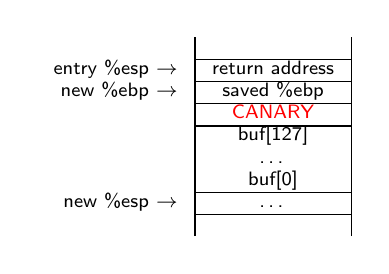
\begin{tikzpicture}
                \node (A) {
                    \scriptsize
                    \begin{tabular}{r|c|}
                        & \\
                        \cline{2-2}
                        entry \%esp $\to$ & return address  \\
                        \cline{2-2}
                        new \%ebp  $\to$& saved \%ebp \\
                        \cline{2-2}
                        & \textcolor{red}{CANARY} \\
                        \cline{2-2}
                        & buf[127] \\
                        & \ldots \\
                        & buf[0] \\
                        \cline{2-2}
                        new \%esp  $\to$& \ldots \\
                        \cline{2-2}
                        & \\
                    \end{tabular}
                };
            \end{tikzpicture}
        \end{tabular}

        \paragraph{Canary value}: 
        \begin{itemize}
            \item[\textsc{Terminator}]: Avec une valeur tel que (0, CR, LF, -1), 
                si l'attaquant veut faire un overflow il doit ajouter un caractère 
                qui est considéré par la plus part des functions comme un caractère
                de fin de String!
            \item[\textsc{Random}]: Soit il doit être très dur à trouver sans
                quoi l'attaquant n'a qu'a inséré cette valeur dans son overflow.
        \end{itemize}

        \paragraph{Limitations}:
        \begin{itemize}
            \item Le canary ne prévient pas des attaques qui overwrite
                un pointer avant le canary
            \item Overflow sur le heap
            \item Malloc/free overflow 
                %TODO

        \end{itemize}


    \item \textbf{Bounds checking}: Prevenir l'utilisation de pointeur invalide.

        \paragraph{Difficulté}: En c, un pointeur n'encode pas d'information
        sur la sémantique de l'usage de ce pointeur. De plus les unions peuvent
        rendre les choses difficiles puisqu'une variables peut être différente chose..

        La solution (qui est weakness puisque l'utilisation d'invalide poiteur est 
        toujours possible) consiste à checker les bornes de la mémoire. Cela
        évite la réécriture arbitraire de la mémoire.

        \begin{itemize} 
            \item[\underline{Contre}]: Nécessite un nouveaux compilateur et donc les l'accès
        aux fichiers sources.
\end{itemize}

        \begin{enumerate}
            \item Electric fences : Ajout à chaque objet dans le heap d'un \textbf{guard page}
                qui cause une page exception quand il est overwrite.
                \begin{figure}[!h]
                    \centering
                \begin{tabular}{|c|}
                    \hline
                    Guard page \\
                    \hline
                    Heap object \\
                    \hline
                \end{tabular}
                \caption{Guard page}
            \end{figure}
                \begin{itemize}
                    \item[\underline{Pour}]: Il ne faut pas changer de compilateur, juste relinker
                        avec une nouvelle version de malloc
                    \item[\underline{Contre}]: Gros overhead pour les objets du heap.
                \end{itemize}
            \item Fat pointer : Modifier la représentation du pointeur pour ajouter
                les informations sur les bornes des objets de cette zone mémoire.

                L'assignation d'une nouvelle valeur à un pointeur peut donc créer une 
                erreur lorsqu'il n'est pas dans les bornes.
                \begin{figure}[!h]
                    \centering
                    \begin{tabular}{|c|m{2cm}|c|c|c|}
                        \cline{1-1}
                        \cline{3-5}
                    4 byte addr & & 4 byte obj\_base & 4-byte obj\_end & 4-byte curr\_adr \\
                        \cline{3-5}
                        \cline{1-1}
                \end{tabular}
                \caption{Représentation fat pointeur}
            \end{figure}
                \begin{itemize}
                    \item[\underline{Contre}]: Couteux de vérifié tout les pointeurs
                        déférencé\ldots surtout que le c veut des performances
                    \item[\underline{Contre}]: Fat pointeur est incompatible avec bcp de
                        programme existant
                \end{itemize}
        \end{enumerate}

    \item \textbf{Non executable memory}: Généralement, on empeche qu'en zone mémoire
        soit exécutable et écrivable! Typiquement, la stack ne sera pas exécutable et
        on ne pourra pas y faire exécuter un code malicieux.
        (\textsc{DEP}, \textsc{NX},\ldots)
        \begin{itemize}
            \item[\underline{Pour}]: Facile à mettre en oeuvre.
            \item[\underline{Contre}]: Dur de générer du code dynamiquement
        \end{itemize}

    \item \textbf{Randomize memory addresses} (Stack ou espace mémoire complet): Les shell-code use souvent des 
        adresses hardcodés, donc en randomisant les adresses c'est plus dur d'avoir
        un pointeur valide.
        (\textsc{ASLR},\ldots)

        \paragraph{Note}: Adversaire peut prendre extraire la randomisation, 
        surtout dans le cas des machines 32bits.
        
\end{enumerate}

En pratique on utilise surtout gcc, la randomization et la mémoire non exécutable.

\subsection{Injection vulnerabilities}
%TODO


\section{Malwares}

Code malicieux qui tourne sur le système d'une victime.

\paragraph{Actions}

Ils peuvent faire à peut près n'importe quoi\ldots cela dépend
surtout des permissions sous lequel ils s'exécutent.
(pop up, endommagé l'hardware, spam, DoS, keylogging, encrypt files)

\paragraph{Time bomb} Les malwares peuvent aussi être retardé en attendant 
qu'une condition arrive.

\subsection{Type de malware}
\begin{description}
  \item[Virus] fragment de code qui se propage à travers des systèmes en s'arrangeant
      pour être \textit{éventuellement} executé. $\to$ infecte en altérant du
      code \textbf{enregistré}
  \item[Worm] programme indépendant qui se prograge/réplique à travers un système
      en s'arrangeant pour être \textit{immédiatement} executé. $\to$ infecte
      en altérant du code qui \textbf{s'exécute}. (pas d'intervention de l'utilisateur)

  \item[$\to$] Les virus et worms sont des malwares qui se propage automatiquement.
  \item[]
  \item[Cheval de Troie (Trojan)] programme utile qui contient un programme malveillant (ou lui-
même par extension).
  \item[Backdoor] accès caché à un ordinateur.
Le Programme permet d'accéder à distance à un système, sans que l'utilisateur le sache.
Ils sont installé par les chevaux de Troie et donc souvent classés comme tels.
  \item[Spyware] programme qui envoie les informations vous concernant à des tiers.
  \item[Adware] programme qui provoque l'apparition d'annonces sur votre écran ou des
    changements des résultats de votre recherche (manipule le navigateur)
  \item[Rootkit] programme qui masque la présence de programmes malveillants sur votre ordinateur.
    Il modifie votre système d'exploitation afin de cacher l'exécution des programmes,
    des fichiers ou des configurations.
\end{description}

\subsection{Virus}

\paragraph{But virus/worm}: Dur à détecter/détruire/désactiver, infection rapide, 
peut réinfecteur d'autre host, facile à créer et indépendant de l'OS. 

\paragraph{Virus problem}
Le virus (comparé au worm) est opportuniste puisque le code n'est pas forcément
exécuté\ldots il le sera si le user effectue une action (ex: démarrer une app,\ldots)

\begin{itemize}
\item \textbf{Les virus Stealth}
    \begin{enumerate}
      \item Simple: le virus comprime le fichier original, et crée un
fichier infecté de la même taille.
      \item Complexe: le virus modifie le système de manière à être
      invisible. Il modifie le fichier routines de lecture afin qu'ils
      ne révèlent pas le virus.
    \end{enumerate}
\item \textbf{Les virus polymorphes}
    Le virus se modifie après chaque infection de manière à rester indétectable.
\end{itemize}

\subsubsection{Période}

\paragraph{La période classique}

Propagation passive à travers l'échange de disquettes. La propagation
est lente et donc le virus à besoin d'être efficace.

\paragraph{La période moderne}

Les virus modernes utilisent Internet pour propager activement et
peuvent infecter la planète en quelques heures. Ils sont souvent,
simple et facile à détecter. Cependant, ils sont efficace, car ils se
propagent beaucoup plus rapidement que le logiciel antivirus ne peut
être mis à jour.

\subsubsection{Propagation}
Quand le virus s'exécute, il cherche des opportunités d'infectés des systèmes
additionnels.

\begin{enumerate}
    \item Une première approche, le virus cherche à altérer les exécutables
        qui se trouve sur \textbf{d'autres système hardware}
    \item Ou bien il altère les pièces jointent au mail pour ajouter une
        copie de lui même.

    \item[Note:] Il peut aussi directement envoyer certain mail
\end{enumerate}

\paragraph{Infection programme}

\begin{figure}[!h]
    \centering
    \scriptsize
    \begin{tikzpicture}[scale=0.7]
        \node (A) {
            \begin{tabular}{|m{3.5cm}|}
                \hline
                Original program instruction\\
                \hline
    \end{tabular}};
    \node (B) [below=1cm of A] {
            \begin{tabular}{|c|m{3.5cm}|}
                \hline
                Virus & Original program instruction\\
                \hline
    \end{tabular}};
    \node (C) [below=1cm of B] {
            \begin{tabular}{|c|m{3.5cm}|c|}
                \hline
                 & Original program instruction & Virus \\
                \hline
    \end{tabular}};

    \node (D) [left= of B] { Point d'entrée };

    \path[->] (D) edge (A.180)
          (D) edge (B.180)
          (D) edge (C.180)
          (C.187) edge [bend right] node [above] {jmp} (C.353)
          (C.7) edge [bend right] node [below] {jmp} (C.173);
      \end{tikzpicture}
    \caption{Programme infecté selon deux variantes possibles}
\end{figure}


\subsubsection{Detection virus}

La détectione est basé sur la \textbf{signature du virus} (byte correspondant
au code malicieux injecté)\ldots 
\begin{itemize}
    \item[$\to$] c'est très utile puisque par nature
        le virus se duplique (et conserve donc sa signature).
\end{itemize}


\paragraph{Création}
Le problème (pour un créateur de virus) est donc 
\begin{enumerate}
    \item de changer son virus
        lorsque sa signature est détecté 
    \item[ou]
    \item changer son apparence gràce à un code \textbf{polymorphic}.
\end{enumerate}


\subsubsection{Polymorphic code}

Le virus se propage en insérant une nouvelle copie \textbf{encrypté} de lui 
même, en variant évidement l'encryption (clé différente ou random padding).

\begin{enumerate}

\item Avec \textbf{Encryption} : elle ne doit pas être \textsc{strong}, juste rapide
simple et \textit{cacher} le virus (= obfuscation).

\begin{figure}[!h]
    \centering
    \scriptsize
    \begin{tikzpicture}[scale=0.7]
        \node (A) {
            \begin{tabular}{|m{6.5cm}|m{3.5cm}|}
                \hline
                Virus & Original program instruction\\
                \hline
    \end{tabular}};

        \node (B) [below=0.4cm of A] {
            \begin{tabular}{|m{1.5cm}|m{1cm}|m{3cm}|m{3.5cm}|}
                \hline
                Decryptor & Key & Encrypted & Original program instruction\\
                \hline
    \end{tabular}};

        \node (C) [below=1cm of B] {
            \begin{tabular}{|m{1.5cm}|m{1cm}|m{1.5cm}|m{1.5cm}|m{3.5cm}|}
                \hline
                Decryptor & Key & Main virus & Encryptor & Original program instruction\\
                \hline
    \end{tabular}};

        \node (D) [below=1cm of C] {
            \begin{tabular}{|m{1.5cm}|m{1cm}|m{3cm}|m{3.5cm}|}
                \hline
                Decryptor & Key 2 & Encrypted 2 & Original program instruction\\
                \hline
    \end{tabular}};

    \draw[->] (B.180) edge[bend right] node[right] {1.} (C.180);
    \draw[->] (B.185) edge node[above right] {2.} (C.170);
    \draw[->] (C.265) edge node[above left] {3.} (D.175);

\end{tikzpicture}

    \captionsetup{singlelinecheck=off}
    \caption[level]{\begin{enumerate}
    \item Décrypte le virus gràce à la clé
    \item Jmp sur le début du code du virus
    \item Dupplique le virus en changeant sa signature avec une encryption différente
    \end{enumerate}}
\end{figure}

\paragraph{Détection}
\begin{itemize}
\item Utiliser une signature plus étroite pour cibler le decryptor. Dans ce cas, il y aura 
plus de \textit{false positives}.
\item Regarder (par analyze static ou en éxécutant) si le code se décrypte lui même.
Certains code non malicieux se décrytpte (ex: decompression).
\end{itemize}

\item Avec \textbf{code rewriter}: l'idée est de se propager en générant une version
sémanticallement différente (au niveau de l'exécution).

\begin{itemize}
\item Renumber register
\item Change order of conditional code
\item Reorder operations not dependent 
\item Replace one low-level algortihm with another
\end{itemize}

\paragraph{Detection}: besoin d'anayser le comportement de l'exécution
\begin{itemize}
\item AV compagnie génère des \textbf{behavioral signature}
\item AV software test if code match with signature
\end{itemize}

\end{enumerate}


\subsection{Infection cleanup}
%TODO

\subsection{Large-scale malware}

\begin{tabular}{m{11cm}m{4cm}}
La propagation est \textbf{plus rapide} que les virus car il 
peut parrallélisé le processus de propagation.

En effet, le worm se propage en s'arrengeant pour être immédiatement exécuté.
&
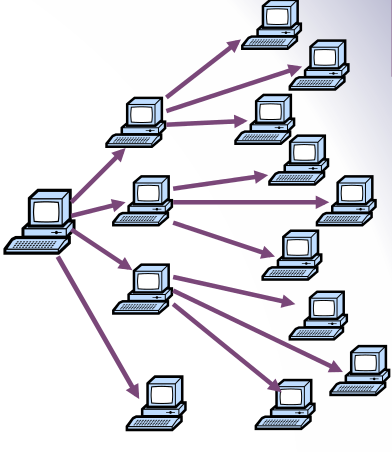
\includegraphics[width=3cm]{img/worm.png}
\end{tabular}

\subsubsection{Worm spread}
Décrit l'épidémié d'infection.

\begin{tabular}{m{6cm}m{6cm}}
\begin{description}
\item[$N$] : population size
\item[$S(t)$] : susceptible host at time $t$
\item[$I(t)$] : infected host at time $t$
\item[$\beta$] : contact rate
\item[$i(t)$] : $I(t)/N$
\item[$s(t)$] : $S(t)/N$
\item[$\to$] : $S = N - I$, $s(t) + i(t) = 1$
\end{description}
&
$$ N = S(t) + I(t)$$
$$S(0) = I(0) = N/2$$

\end{tabular}

\paragraph{In continuous time}:

\begin{tabular}{m{4cm}m{0.5cm}m{4cm}m{0.5cm}m{4cm}}
$$ \frac{dI}{dt} = \beta I \frac{S}{N}$$
&==&
$$\frac{di}{dt} = \beta i (1-i)$$
& == &
$$i(t) = \frac{e^{\beta t}}{1+ e^{\beta t}}$$
\end{tabular}

\begin{figure}[!h]
\centering
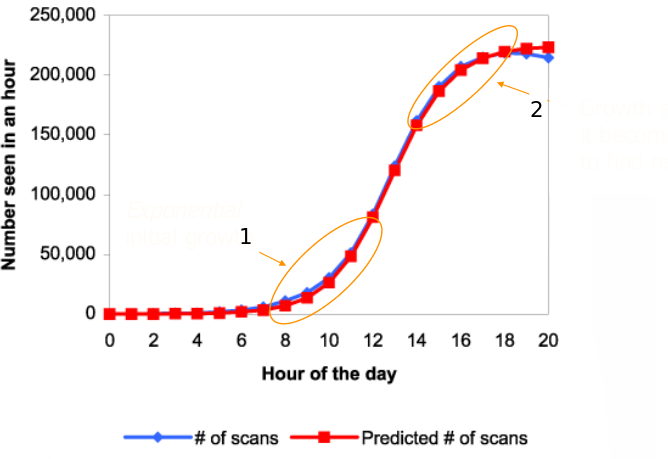
\includegraphics[width=11cm]{img/wormspread.png}
\caption{1. Initial exponential growth, 2. Grow slow as it become harder to find new victims}
\end{figure}


%TODO slammer stuxnet




\section{Cryptographie}
La cryptogaphie a pour but d'assurer plusieurs propriétés:
\begin{itemize}
	\item \textbf{Confidentialité} : seuls les acteurs de la communication peuvent
	savoir ce qui est dit.
	\item \textbf{Intégrité} : assurer au destinataire que le message reçu n'a pas
	été modifié.
	\item \textbf{Authentification} : vérifier l'identité de celui qui a envoyé le
	message.
	\item \textbf{Non-répudiation}: pouvoir convaincre un tier que ce qui a été 
	dit est correct.
\end{itemize}

\paragraph{Terminologie}
\begin{description}
	\item[Algorithm d'encryption]: Transforme un texte clair en texte
	chiffré à l'aide d'une clé. 
	\item[Cryptographie à clé asymmétrique ou clé publique]: une clé
	différente est utilisée pour crypter/décrypter. 
	\item[Cryptographie à clé symmétrique ou partagée]: la même clé est
	utilisée pour crypter/décrypter. 
	\item[Clé à usage unique]: on utilise une nouvelle clé pour chaque 
	message. (ex: mail encrypté)
	\item[Clé à usage multiple]: la même est utilisé pour encrypter
	plusieurs messages. (ex: SSL)
\end{description}

\subparagraph{Note}: Il est important d'utiliser des algorithmes publiquement 
connus pour que les failles puissent vite être découverte.

\paragraph{Attention}

La cryptographie est la base pour beaucoup de sécurité mais ce n'est pas:
\begin{enumerate}
	\item a solution à tout les problèmes de sécurité.
	\item privacy : contrôle des informations personnels.
	\item stéganographie: la science qui consiste à cacher de information.
	\item Encoder et decoder.
\end{enumerate}

\paragraph{Cryptanalyse}
Elle est à différencier de la cryptananlyse qui constiste à:
\begin{itemize}
  \item Science qui confirme ou infirme la sécurité d'un système de cryptographie.
  \item Prouver l'insécurité d'un système de cryptographie.
\end{itemize}

La cryptotologie est la science qui combine cryptographie et la
cryptanalyse.



\subsection{Sécurité Sémantique}
\begin{itemize}
    \item $EXP(0)$, $EXP(1)$ define as :

        \begin{tabular}{cc}
            Clé symmétrique & Clé asymmétrique \\
            \scriptsize
            \begin{tikzpicture}
                \node[draw, rectangle, minimum height=1cm] (A) [initial, initial text={b}] {\begin{tabular}{c}
                    Chal.\\ $k \leftarrow K$ \end{tabular}};
                \node[draw, rectangle, minimum height=1cm] (B) [right=4cm of A] {Adv. A};
                \node (C) [below=of B] {};

                \draw[->] ([yshift=1ex]A.east) edge node[above] { $m_0, m_1 \in M : | m_0 | = | m_1 |$ } ([yshift=1ex]B.west);
                \draw[->] ([yshift=-1ex]B.west) edge node[below] {$c \leftarrow E(k, m_b)$} ([yshift=-1ex]A.east);

                \draw[thick] ($(A.north west)+(-0.25,0.25)$) rectangle ($(B.south east)+(0.25,-0.25)$);
                \draw[->] (B.south) edge node[left] {$EXP(b)$} (C);
            \end{tikzpicture}
	&
            \scriptsize
        \begin{tikzpicture}
                \node[draw, rectangle, minimum height=1cm] (A) [initial, initial text={b}] {\begin{tabular}{c}
                    Chal.\\ $(pk, sk) \leftarrow G()$ \end{tabular}};
                \node[draw, rectangle, minimum height=1cm] (B) [right=4cm of A] {Adv. A};

                \node (C) [below=of B] {};

                \draw[->] ([yshift=3ex]A.east) edge node[above] {$pk$} ([yshift=3ex]B.west);
                \draw[->] ([yshift=-1ex]B.west) edge node[above] { $m_0, m_1 \in M : | m_0 | = | m_1 |$ } ([yshift=-1ex]A.east);
                \draw[->] ([yshift=-3ex]A.east) edge node[below] {$c \leftarrow E(pk, m_b)$} ([yshift=-3ex]B.west);
                \draw[->] (B.south) edge node[left] {$EXP(b)$} (C);

                \draw[thick] ($(A.north west)+(-0.25,0.25)$) rectangle ($(B.south east)+(0.25,-0.25)$);
            \end{tikzpicture}
	\\
\end{tabular}
 
\item For $b=0,1$ : $W_b = [$ event that $EXP(b) = 1 ]$
\item $Adv_{ss}[A, E] = | Pr[W_0] - Pr[W_1] | \in [0, 1]$
\end{itemize}

   
\begin{center}
    $\to$ E est \textbf{sémantiquement sécurisé} si $\forall$ attacker
efficace A : $Adv_{ss}[A,E]$ est négligeable. (négligeable n'est pas
vraiment défini)
\end{center}



\subsection{Cryptographie à clé symmétrique}

Un cipher défini pour (K, M, C) avec une paire d'algorithme \textit{efficace} (E, D)
\begin{itemize}
	\item M : l'ensemble des messages
	\item K : l'ensemble des clés
	\item C : l'ensemble des codes
	\item[]
	\item E : $K \times M \to C$
	\item D : $K \times C \to M$
	\item[tel que]
    $$\forall m \in M,k\in K:\quad D(k,E(k,m))=m$$
\item[$\to$] E est souvent randomize alors que D est toujours deterministique.
\end{itemize}

\paragraph{Cypher types}: 

\begin{figure}[!h]
\begin{tabular}{|c|p{3cm}|p{8cm}|}
    \hline
    par stream & act on the plaintext one symbole at a time & \begin{itemize}
        \item[+] High speed rate, cheap hardware implementations 
        \item[-] Security analysis is not well established
    \end{itemize}
    \\
    \hline
    par block & act on the plainttext in blocks of symbols & \begin{itemize}
        \item[+] Security analysis is well established
        \item[-] Need software implementation
    \end{itemize}
    \\
    \hline
\end{tabular}
\caption{Cypher type}
\end{figure}

\paragraph{Modèle d'assaillant}:

\begin{tabular}{|l|p{11cm}|}
    \hline
    \textbf{Attack} & \textbf{Attacker acces} \\
    \hline
	Ciphertext-only :& Cipertext de un ou plusieurs message encrypté avec la même clé. \\
	\hline
	Known-plaintext :& Paires ciphertext-plaintext encrypté avec la même clé.\\
	\hline
 Chosen-ciphertext :& Un oracle de décryption : il peut choisir
des ciphertext (basé sur la même clé) et recevoir le plaintext
correspondant.\\
	\hline
	Chosen-plaintext attack:&  Un oracle d'encryption : 
	il peut choisir un plaintext et recevoir le ciphertext correspondant
	basé sur la même clé.
	(Plus puissant que le CCA) \\
	\hline
\end{tabular}


\subsubsection{Stream Ciphers}
Les stream ciphers consiste à agir sur le plaintext symbole par symbole.

\paragraph{\textbf{One Time Pad} (Vernam)}

\begin{itemize}
    \item $M=C=\{0,1\}^n$
    \item $K=\{0,1\}^n$ tel que k est une clé random de la taille du message
    \item[] \begin{align*}
            E(k,m)&=k\oplus m \\
            D(k,c)&=k\oplus c \\
        \end{align*}
    \item[$\to$] On a bien : $D(k,E(k,m))=D(k,k\oplus m)=k\oplus(k\oplus)=(k\oplus k)\oplus m=0\oplus m=m$

    \item[]

    \item[Problème] : la clé doit être aussi longue que le message. 

        \paragraph{Pseudo random key} : 
        Génère une clé pseudo random d'une taille donné (celle du msg) 
        à partir d'une clé potentiellement plus petite.
        $$m\oplus PRG(k) \to C$$

        Un stream utilise une clé à \textbf{usage unique}. En effet supposons:
        $$\left\{
            \begin{array}{rcr}
                C_1 & = & m_1 \oplus PRG(k)\\
                C_2 & = & m_2 \oplus PRG(k)\\
            \end{array}
            \right. $$
            Un attacker peut faire $C_1 \oplus C_2 \to m_1 \oplus m_2$ grâce à la 
            redondance des charactères (probabilité d'utilisation d'un lettre 
            n'est pas la même pour toute les lettre), il peut retrouver $m_1,m_2$


\end{itemize}

\subsubsection{Block Ciphers}

Ils agissent sur le plaintext bloc par bloc de symbole. 
Ils fonctionnent par itération, càd que les blocks chiffrés sont
utilisé comme input pour le chiffrement des blocks suivants.

\paragraph{\textbf{Feistel Network}}

\begin{figure}[!h]
    \centering
    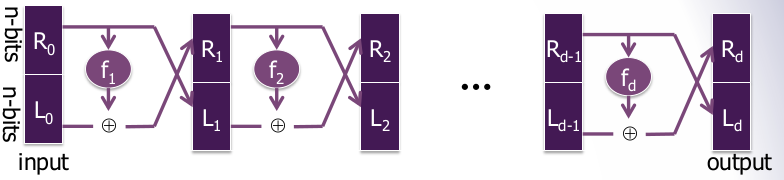
\includegraphics[width=\linewidth]{img/feistel.png}
    \caption{Feistel principle}
\end{figure}

\begin{itemize}
    \item[Given] $f_1,\cdots, f_d$ : $\{0, 1\}^n \to \{0, 1\}^n$
    \item[Build] $F: \{0,1\}^{2n} \to \{0, 1\}^{2n}$

    \item[] 
    \item[] 
        \begin{center}
            \begin{tabular}{m{5cm}m{0.5cm}m{5cm}}
            Construct cyphertext & $\Rightarrow$ & Construct plaintext \\
            \hline
            {$\!\begin{aligned}
                R_i &= f_i ( R_{i-1} ) \oplus L_{i-1}\\
                L_i &= R_{i-1}\\
            \end{aligned}$}
            & $\Rightarrow$& 
            {$\!\begin{aligned}
                R_{i-1} &= L_i\\
                L_{i-1} &= R_i \oplus f_i ( L_i)\\
            \end{aligned}$}
            \\
            \centering 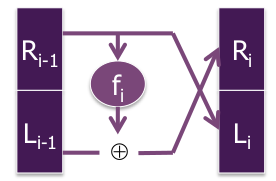
\includegraphics[width=2cm]{img/feistel1.png} & $\Rightarrow$ &
            \centering 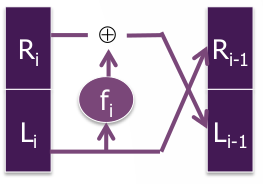
\includegraphics[width=2cm]{img/feistel2.png} \\
        \end{tabular}
        \end{center}
\end{itemize}


\paragraph{Example}:
\begin{itemize}
    \item \textsc{DES} : 16-round feistel network.

        \begin{figure}[!h]
            \begin{tabular}{m{6cm}m{8cm}}
                \begin{description}
                    \item $ f_1,\cdots,f_{16}: \{0, 1\}^{32} \to \{0, 1\}^{32}$
                    \item $f_i(x) = F(k_i, x)$
                \end{description}
        &
            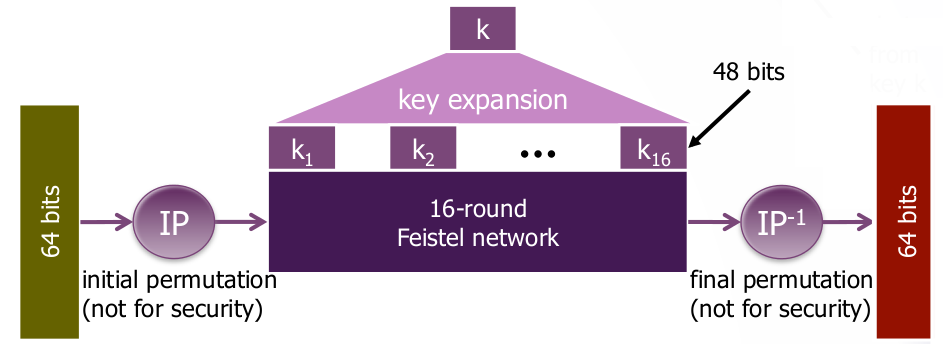
\includegraphics[width=9cm]{img/DES.png}
        \end{tabular}
            \caption{DES principle}
        \end{figure}

	\item 3DES: par block de 64 bits et une clé de 168 bits ($3 \times 56$)
	    $$ 3E( (k_1, k_2, k_3), m) = E(k_1, D(k_2, E(K_3, m)))$$

	\item AES: par block de 128 bits et une clé de 128,192,256 bits
\end{itemize}


\subsubsection{Problème Crypto clé partagé}
\begin{itemize}
	\item Une clé compromise signifie que quelqu'un qui interceptait les 
	messages chiffré va pouvoir les décrypter.
	\item La distribution de la clé 
\end{itemize}


\subsection{Tiers de Confiance}

Stocké un clé mutuel pour chaque utilisateur d'un réseau signifie
qu'il va y avoir $O(n^2)$ clé dans le systéme ce qui n'est pas très 
efficace. On utlise alors un tier qui va générer les clés partagées
à partir des clés des utilisateurs.$\to$ Chaque utilisateur 
doit seulement retenir une clé.


\subsubsection{Toy Protocol}
Supposons que Alice a une clé $k_A$ et Bob a une clé $k_B$.
Alice veut une clé partagé avec Bob.
\begin{enumerate}
	\item Alice prévient le tier de confiance qu'elle veut une clé
	partagé avec Bob.
	\item Le tier de confiance va choisir de façon aléatoire une 
	clé $k_AB$.
	\item Le tier de confiance envoie à Alice
		\begin{itemize}
			\item $E(k_A,''A,B'' || k_AB)$
			\item Un ticket : $E(k_B,'''A,B''||k_AB)$
		\end{itemize}
	\item Alice va envoyer à Bob le ticket.
	\item Alice et Bob vont pouvoir decrypter ce qui a été
	envoyer par le tier de confiance grâce à leurs clé respective.
\end{enumerate}

Ce protocol est sécurisé contre les eavesdroppers mais vulnérable au 
attaque man-in-the-middle.                                              

\paragraph{Eavesdroppper}
Tout ce que eavesdropper voit c'est 
$E(k_A,''A,B''||k_AB)\quad;\quad E(k_B,'''A,B''||k_AB)$.

\subparagraph{Note:} $(E,D) \rightarrow$ eavesdropper learns nothing about $k_AB$


\subsection{Crytographie à clé asymétrique}

Chaque acteur va générer une paire clés (privé/publique).
\begin{enumerate}
	\item Le sender encrypte en utilisant une clé publique.
	\item Le receiver décrypte en utilisant une clé privée.
    \item[$\to$] Seul la clé privée doit être secrète.
\end{enumerate}

\paragraph{Cipher de clé publique} est composé de 3 algos:
\begin{itemize}
	\item G() : un algo aléatoire qui génére une paire de clé (PK,SK)
	\item E(PK,m) : un algo aléatoire qui prend $m\in M$ et une
	clé PK qui renvoie $c \in C$
\item D(SK,c) : algo deterministe qui prend $c \in C$ et renvoie
    $m \in M \ ou \ \perp$
\item[]
\item[Attention]
    Le cipher doit aussi respecté la propriété de consistance 
    $$\forall(PK,SK)\ retourné\ par\ G:\quad D(SK,E(PK,m))=m\quad \forall m \in M$$
\end{itemize}

\subsubsection{Etablir un secret partagé}
Pour que Alice et Bob partage un secret:

\begin{enumerate}
	\item Alice génére une paire clé (pk,sk) et envoie (''Alice'',pk) à Bob
	\item Bob choisit un secret  $x \in \{0,1\}$
	\item Bob encrypte x avec pk (retourne c) et envoie (''Bob'',c)
	\item Alice décrypte le message de Bob avec sk et connait x.
\end{enumerate}

Cette façon est sécurisé contre les \textbf{eavesdroppers} mais pas contre le 
\textbf{man-in-the-middle}. En effet le MiTM peut se faire passer pour
Alice quand il communique avec Bob et inversément.

\begin{figure}[!h]
    \centering
    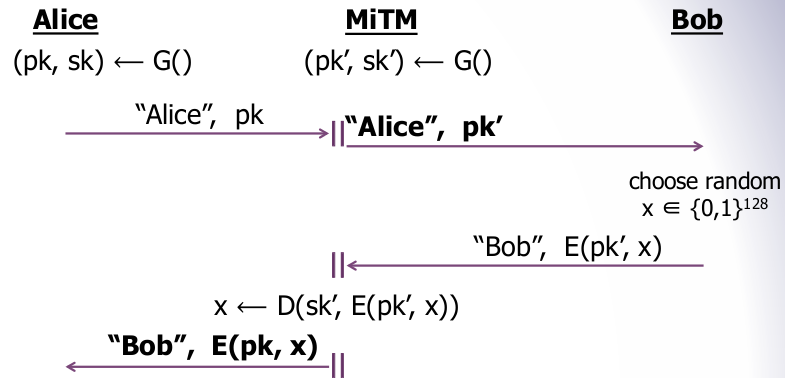
\includegraphics[width=10cm]{img/asyMITM.png}
\caption{MitM attack for asymmetric}
\end{figure}

\subsubsection{Trade-offs}

La crypto à clé publique demande plus de calcul que la crypto à clé
partagé.

\subsubsection{RSA Algorithm}

C'est l'algorithme à clé publique qui est le plus utiliser. Son
implémentation en hardware est 1000 fois plus lente que pour le DES
mais pour l'instant personne n'y a trouvé de faille.

\begin{itemize}
	\item La paire de clé est dérivé de nombre premiers.
	\item Le plaintext est considéré comme un très grand nombre
	binaire.
	\item Pour pouvoir casser, l'encryption il faut pouvoir factorisé
	de très gros nombre (pour l'instant n'a pas l'air d'être dans P)
\end{itemize}


\paragraph{Theoreme d'Euleer}
\begin{itemize}
    \item $\phi(n)$ = $\{ a | 0 < a \le n$ AND $a$ premier avec $n \}$ (GDC avec n = 1)
    \item[$\to$] Le théorème d'Euler nous dit $a^{\phi(n)}\equiv 1\ mod \ n$ pour
	n'importe quelle $a$ premier avec n.
\end{itemize}

\paragraph{Generation de la paire}
La génération de la paire de clé se fait avec l'indicatrice d'Euler.
\begin{enumerate}
	\item Choisir deux nombre premiers $p$ et$q$
	\item Calculer le modulus $n = p\times q$
	\item Calculer  $\phi(n)=(p-1)(q-1)$ 
	\item Choisir $e$ tel que $1<e<\phi(n)$ avec
	$e$ et $\phi(n)$ premier entre eux. 
	\item Determiner $d$ tel que $d\equiv\ e^{-1}\ mod \ \phi(n)$
    \item We have that $d\times e\equiv 1\ mod\ \phi(n)$
\end{enumerate}

$$\Rightarrow \textrm{La clé publique = (e,n) et la clé secrète = (d,n)}.$$

\paragraph{Encryption/Decryption}
$M$ est changé en entier $m$ tel que $0 \le m < n$.\\

\begin{tabular}{m{3cm}m{12cm}}
Encryption (e,n)
&
\begin{itemize}
	\item $c\equiv\ m^e\ mod\ n$
	\item  \begin{enumerate}
		\item $m^e\equiv\ (m^2\ mod\ n)^{(e/2)}\ mod\ n$ si $e\equiv\ 0\ mod\ 2$
		\item $m^e\equiv\ (m^2\ mod\ n)^{(e-1)/2))}\ mod\ n$ sinon
	\end{enumerate}
\item[Note]: On fait les puissance avec les racines carré pour aller plus vite.
\end{itemize}
\end{tabular}


\begin{tabular}{m{3cm}m{12cm}}
Décryption (d,n)
&
\begin{itemize}
    \item $m\equiv\ c^d\ mod\ n$.
    \item 
        $\begin{array}{rcr}
            c^d\ mod\ n & \equiv & (m^e\ mod\ n)^d\ mod\ n\\
            & \equiv & m^{e\times d}\ mod\ n\\
            & \equiv& m^1\ mod n
        \end{array}$

    \item[Note]: La dernière étape fonction grâce au théorême de Euler.
\end{itemize}
\end{tabular}


\paragraph{Encryption hybrid}
Pour encrypter un message tel que m > n, il faut utiliser un encryption
hybrid. Cela consiste à encrypter la clé symmétrique avec RSA, puis 
d'utiliser cette clé pour encrypter.

\paragraph{Signature}
Pour signer un message, il faut l'encrypter avec la clé privé.
Le message pourra être décrypter avec le clé publique.

\subsubsection{Trapdoor Function}

Une trapdoor function, $f: X \to Y$ est une fonction qui facile à
calculer dans un sens mais difficie de calculer dans le sens opposé
sans information supplémentaire.

\begin{itemize}
	\item G() : randomisation de clé (pk, sk)
	\item F(pk, ) : define $f: X \to Y$
    \item F$^{-1}$(sk, ) : define $f: Y \to X$
	    
    \item[$\Rightarrow$] Si f est une trapdoor function alors il existe un 
	secret y tel que avec f(x) et y il est facile de trouver x
\end{itemize}

%TODO encryption from TDF

\subsection{Diffie-Hellman Echange de clé}

Le probléme de la crypto à clé partagé est de savoir comment
distribuer le clé partagé. Diffie-Hellman permet de régler ce
problème sans forcément utiliser un tier de confiance!

\paragraph{Fonctionnement}
Supposons que l'Alice et Bob veulent se mettre d'accord sur 
un secret.
\begin{enumerate}
	\item Alice choisit un nombre premier $g$ ($\ge 512bits$)
	\item Alice choisit $g<p$ tel $g$ est une racine primitive de $p$
	 \begin{description}
			\item[Racine primitive]: $g$ est une racine primitive de $p$
			si $\forall n \in \{1,...,p-1\} \exists k : n =g^k\ mod\ p$

			\item[] Ex: 2 est une racine primitive de 5, $2^0=1,2^1=2,2^2=4,2^3=3\ mod\ 5$
		  \end{description}
	\item Alice et Bob se mettent d'accord pour utiliser g et p
	\item Alice choisit un nombre A et Bob choisit un nombre B
	\item Alice envoie $g^A\ mod\ p$ à Bob et Bob envoie $g^B\ mod\ p$
	\item Le secret partagé devient $g^{AB}\ mod\  p$
    \item[]
    \item[$\Rightarrow$] Alice peut calculer $g^{AB}\ mod\ p$ car elle connait A:$$g^{AB}\ mod\ p=(g^B\ mod\ p)^A\ mod\ p$$
\end{enumerate} 


\paragraph{Eavesdropper}
Le eavesdropper connait $g^A\ mod\ p$ et $g^B\ mod\ p$, il peut calculer
$g^{A+B}\ mod\ p$ mais ça ne l'aide pas. 

\paragraph{Note:} Cette façon de faire est vulnérable au man-in-the-middle.
La sécurité vient du fait qu'il va être difficile de trouver A (B) à partir
de $g^A\ mod\ p$


\subsection{Authentification}

Pour pouvoir prévénir les attaque \textbf{man-in-the-middle}, il faut
que le canal de communication soit authentifier. Cela se fera grâce à
SSL/TLS.

\subsection{Résistance au collision}

\subsubsection{Fonction de hash cryptographique}

Ce sont des fonction qui sont difficile à inverser $h: \{0,1\} * \to \{0,1\}^n$\\
Ces fonctions ont les propriétés suivantes:
\begin{description}
	\item[One way hash function]: Pour une valeur de hash y, il devrait être
	impossible de trouver un message $m$ tel que $h(m)=y$

	\item[Collisions resistance]: Il devrait être impossible de trouver 
	2 messages différents $m_1$ et $m_2$ tel que $h(m_1)=h(m_2)$

	\item[Random oracle value]: $h(m)$ est indistinguable d'un valeur de 
	n-bit. Un attacker doit avoir dur à modifier un message sans
	changer la hash value. 

\end{description}
Les example de fonction sont SHA(Secure Hash Algorithm) et MD(Message
Digest)

\paragraph{Le paradoxe de l'anniversaire}
Dans un groupe de 23 personnes, la probabilité d'avoir au moins 2 
personnes nés le même jour est à peu prés 50\%.

\subsubsection{Generic attack}
For $H: M \to \{0, 1\}^n$ (message de n bits)

\begin{lstlisting}[mathescape]
do 
    Choose $2^{n/2}$ random elements in M: $\{m_1,..., m_2^{n/2}$
    For $i$ = 1,..., $2^{n/2}$ compute $t_i = H(m_i) \in \{0,1\}^n$
    Look for a collision ($t_i = t_j$).
while(not found)
\end{lstlisting}

\begin{center}
On s'attend à une moyenne de $2$ itérations, soit $2^{\frac{n}{2}}$ essai.
Complexité spatial/temporel = $\bigoh(2^{\frac{n}{2}})$
\end{center}


\subsection{MAC}
Les MAC (Message Authentification code) sont utilisés pour s'assurer 
de l'\textbf{intégrité} d'un message.


Ils sont définis par deux algos I=(S,V) qui agissent sur
\begin{itemize}
	\item $K$ : l'ensemble des clés.
	\item $M$ : l'ensemble des messages.
	\item $T$ : l'ensemble des Tag.
    \item[]
    \item $S(k, m) = t \in T$
    \item $V(k, m, t) = \{true, false\}$
    \item[]
    \item[Consistency]: $\forall k \in K, \forall m\in M\quad V(k,m,S(k,m))='yes'$
\end{itemize}

$\Rightarrow$ Un MAC est considéré comme sécurisé si un attacker ne
peut pas produire une paire message/tag valide meme en ayant une paire
valide.

\subsubsection{Pseudo Random Function}

Pour une fonction $F:K \times Y\to Z$ définir un MAC $I_F =(S,V)$
\begin{itemize}
	\item S(k,m) := F(k,m)
	\item V(k,m,t) : renvoie `yes' si t = F(k,m), `no' sinon
\end{itemize}
$I_F$ est sécure si Y est très large $(2^80)$

\subsubsection{Hash-MAC}

C'est MAC le plus utilisé sur internet. Le MAC est construit à partir 
d'une fonction de hash $$HMAC: S(k,m)=H(k\oplus opad || H(k\oplus ipad||m))$$

où opad et ipad représente le padding et H est la fonction de hash.
Les fonctions de hash les plus utilisé sont SHA256 (output de 256 bits)
et SHA1 (output 160 bits)

\paragraph{SHA-256} Le message est découpé en bloc, chaque bloc 
hashé et utilisé pour hashé les suivants.

\paragraph{Insecure MAC construction}
%TODO

%TODO: bouge récap. Question à KABA : les ciphers c'est bien pour les clés symm/asym ?
\subsection{Récap}

\begin{tabular}{|c|c|c|c|}
\hline
Algo&Type&taille de clé(bits)&taille de bloc(bits)\\
\hline
3DES&clé partagée&112,168&64\\
\hline
DES&clé partagée&64 (8 ignorés)&64\\
\hline
AES&clé partagée&128,192,256&128\\
\hline
RSA&clé publique&1024,2048,4096&\\
\hline
\end{tabular}

\section{Network Attacks}

\subsection{Exploits on the web}

\paragraph{Exploits}

La plupart des logiciels contiennent des défauts.
Ces bugs peuvent être exploitées par des pirates.
Un `exploit' est une méthode ou un script qui permet d'exploiter les bugs.
Le plus intéressant sont exploits sur les serveurs.
Ils peuvent se faire à distance et les serveurs ont
souvent des privilèges plus élevés.

%TODO tabular avec different attack selon les layers

\subsubsection{Directory Traversal}

Les documents du serveur Web sont accessibles à partir d'une racine. Si le serveur ne vérifie pas l'URL,
nous pouvons accéder à d'autres fichiers.

\paragraph{Exemple classique}: traversée de répertoire.
\begin{itemize}
  \item \verb|../../../../|
  \item Scripts faibles.
\end{itemize}

\paragraph{Protection}

Pour éviter le Directory Traversal, certaines application web vérifie
la chaîne : \verb|..| et \verb|../..| et \verb|/| dans l'URL.
Cependant, ces applications sont encore vulnérables au encodage ``pour
cent'' de l'URL (\verb|?%2e%2e/| qui est à \verb|../,?..%2F| qui est de
\verb|../..|.), mais aussi l'encodage UTF8, etc.


$\Rightarrow$ La Sécurité de l'application dépend du codage autorisé
par le serveur web.

\subsubsection{Cross-Site Scripting}
Le «Cross-site» consiste à insérer un script dans une page Web.
Souvent, la script lui-même est situé
sur un autre serveur, c'est du "Cross-site scripting".
(\textit{Example : \texttt{<script src=http://www.evilsite.com/hack.js>} })

\paragraph{Dangers}:
\begin{itemize}
  \item Réorientation de la session (par exemple, sur une copie du site original).
  \item Afficher de fausses informations.
  \item Afficher des formulaires de collecte de données (phishing).
  \item Vole des cookies.
\end{itemize}

\subsubsection{Phishing}

Le but est d'obtenir des informations et identification se faisant
passer pour une entité digne de confiance.

Le plus souvent par email, l'adresse ressemble à
l'adresse valable. Par exemple \url{www.mybanck.com} ou
\url{http://www.mybank.com.example.com}.

On peut aussi avoir une image avec un lien hypertexte.

\subsubsection{SQL Injection}
Exploitation d'une faille de sécurité d'une application interagissant avec une base de données, en
injectant une requête SQL non prévue par le système et pouvant compromettre sa sécurité.


\subsection{Denial of Service}

Le déni de service consiste à empecher quelqu'un d'utiliser un service.
Il y a deux approches possibles :

\begin{itemize}
	\item Déni de service dû a une faille dans le programme(ex:
	input qui force le serveur a crash)
	\item Déni de service dû à l'épuisement des ressources du système
	(ex:while(1);) 
\end{itemize}

\subsubsection{DoS et OS}

Différentes façon de faire un DoS dans un systeme comme écrire 
sur tout le disque dur ou créer plein de processus\\
$\rightarrow$ Défense en isolant les utilisateurs et imposant des quotas.

\subsubsection{Dos et Réseau}

Pour faire un DoS sur l'accès internet d'une victime, il suffit de lui 
envoyer plein de packet. Pour pouvoir faire cela, l'attacker a besoin
de ressource:

\begin{itemize}
	\item Il lui faut au moins un bande passante supérieur au lien 
	le plus faible de la connection internet de la victime.
	\item Ou bien pouvoir surchager le routeur qui a la capacité de 
	calcul la plus faible.
\end{itemize}

\subsubsection{Ping of death}

La taille normale d'un Ping est de 64 octets (84 avec en-tête).
On envoie des paquets IP qui dépassent la taille légale maximale (65535 octets).
C'est l'une des premières attaque par déni de service.
Unix, Linux, Mac, Windows, imprimantes et routeurs étaient vulnérables ($<1997$).

\paragraph{TCP Handshake}:
L'établissement d'une connexion TCP se fait par un handshaking en trois temps:
\begin{enumerate}
  \item Le client envoie un segment $\syn(x)$ au serveur, avec $x$ son sequence number.
  \item Le serveur lui répond par un segment $\syn+\ack(y,x+1)$, avec $y$ son sequence number.
  \item Le client confirme par un segment $\ack(x+1,y+1)$.
\end{enumerate}

\subsubsection{Syn-Flooding}

\begin{enumerate}
    \item On envoit un grand nombre de demandes ouverture de connexion TCP ($\syn$).
    \item À la réception du paquet $\syn$, le serveur crée une ``demi-connection''
        qui utilise du CPU et une entrée dans le TCB (transmission control block)
        Une fois le TCT rempli, le serveur ne plus plus accepter de nouvelle connections.

        $\to$L'attaquant peut forger l'adresse source de ses paquets $\syn$ rester anonyme.
\end{enumerate}

\paragraph{Protection}
Les versions récentes des systèmes d'exploitation (Windows, Unix)
sont protégés contre de telles attaques.
Protections contre les $\syn$ Flooding :
\begin{itemize}
  \item Augmenter la taille de la file d'attente.
  \item Réduire délai pendant lequel le serveur attend un $\ack$.
  \item Dropper le plus ancien $\syn$ dans la file d'attente.
  \item Filtrage, par exemple sur les adresses IP (en identifiant les mauvais acteurs)
  \item $\syn$-Cache: cache le $\syn$ et envoyer un $\syn$ / $\ack$. Si les $\ack$ arrive, une connexion complète
    est créée.
  \item $\syn$-Cookies: Une fois que la file d'attente de connexion est presque rempli, le serveur utilise
    les cookies $\syn$.

\end{itemize}


\subsubsection{Smurf Attack}
Le but est de noyer la cible à l'aide d'amplificateurs de circulation.

Cas typique: ICMP echo-request (ping).
\begin{itemize}
  \item Le pirate envoie un paquet de ping avec l'adresse cible
comme adresse source.
  \item La machine ``pings'' envoie sa réponse à la cible.
  \item Si le pirate envoie le paquet à une adresse de diffusion
    (broadcast) , toutes les machines du réseau répondront à
    la cible.
\end{itemize}
Protection:
\begin{itemize}
  \item Configurer les hôtes et les routeurs individuels afin de ne pas répondre aux requêtes ping à
    une adresse de broadcast.
  \item Configurer les routeurs afin de ne pas transmettre les paquets dirigés vers des adresses de
    broadcast.
\end{itemize}

\subsubsection{DNS lookup}
L'attacker profite du fait que les réponses DNS soit beaucoup plus
grande. L'attacjer va donc envoyer des requêtes DNS avec l'IP 
de la victime.\\
$\rightarrow$ Autre techniques d'amplification car avec des
petit paquet, on peut en générer de gros.

\subsubsection{DDoS (Distributed Denial of Service)}

Pour augmenter l'efficacité du déni de service, les pirates vont pirater plusieurs machines et installer
des agents.

\begin{itemize}
	\item L'attacker est appelé le \textbf{Botmaster} et il dispose de plusieurs
	serveur appelés \textbf{Serveur-Maître} ou Commande\&Controle
	\item Les C\&C envoient des ordres à des machines infectées
	appelées \textbf{Bots} selon les désirs du Botmaster.
\end{itemize}

La puissance (bande passante) de l'attaque est multipliée par les agents.
Il est plus difficile de retracer les pirates (2 couches intermédiaires).
Puisque l'attaque provient de plusieurs sources, elle est beaucoup plus 
difficile à filtrer.

\paragraph{Combattre bots} 
\begin{itemize}
	\item  Une approche serait de trouver l'IP du C\&C et le descendre.
	 $\rightarrow$ L'attacker peut utiliser un nom de domaine pour pouvoir
	 changer d'IP
	\item  On pourrait alors saisir le nom de domaine $\rightarrow$
	L'attaker change de nom de domaine et le bot génère un liste
	de nom possible.
\end{itemize}


\subsubsection{RST injection}

L'idée est d'envoyer enormément de RST packet pour fermer toute les connections ouvertes
par le serveur.

\subsection{Spoofing}
\subsubsection{IP Spoofing}
Dans certains cas, l'adresse IP source est utilisé pour autoriser une connexion.
Les routeurs et les pare-feu peuvent filtrer les paquets en fonction de leur source.
Certains programmes (rlogin, rsh) peuvent
autoriser certaines sources à se connecter sans authentification.
Il est facile d'usurper l'adresse source d'un paquet et d'abuser de la confiance de cette source.
La réponse à un message forgé est envoyé à l'adresse falsifiée.
Facile à utiliser avec les protocoles basés sur UDP.

\subsubsection{TCP/IP Spoofing}
Il est difficil de faire une attaque spoofing dans une connection 
TCP car il faut utiliser le bon numéro de séquence.

\subsubsection{TCP/IP Spoofing Dans un LAN}
En sniffant le traffic circulant dans la LAN, l'attacker pourra
facilement les numéros de séquences qu'il doit utiliser 
pour spoofer une connection TCP.

\subsubsection{TCP/IP Spoofing De l'extérieur}
Prédiction de l'ISN (Incremental Sequence Number):
La norme originale (RFC 793) exige que l'ISN est incrémenté une fois tous les quatre microsecondes.
Dans certaines implémentations TCP simples le prochain ISN peut être prédit.
La procédure du Hacker pour prédire l'ISN:
\begin{itemize}
  \item Il ouvre quelques liens authentiques (par exemple SMTP) pour obtenir les échantillons
    d'incrémentation d'ISN actuels.
  \item Il lance sa connexion forgée en utilisant le dernier ISN plus un incrément obtenu à partir de ces
    échantillons.
  \item Il peut lancer plusieurs connexions forgés avec des incréments différents en espérant qu'au
    moins un d'entre eux est correct.
\end{itemize}

\subsubsection{ARP Spoofing}
ARP = Address Resolution Protocol.
L'ARP est un protocole qui permet de trouver une adresse de la couche 2 (Ethernet) à partir d'une
adresse de couche 3 (IP). Il Très simple et non sécurisé:
\begin{itemize}
  \item Un client demande qui connaît l'adresse Ethernet 10.1.2.3?
  \item Une personne répond 10.1.2.3 a l'Adresse Ethernet 010203040506.
\end{itemize}
Il est facile de forger des réponses (même les non-sollicité) pour rediriger le trafic!

\subsection{Sniffing}
De nombreux protocoles utilisent l'authentification par texte claire (pas d'encodage).
Par l'écoute du traffic sur une partie du réseau, nous pouvons obtenir les noms d'utilisateur et mots de
passe. Un mot de passe permet d'accéder à un ordinateur distant à partir de laquelle nous pouvons
renifler à nouveau et obtenir des nouveaux mots de passe.

\subsection{Session Hijacking}
\subsubsection{Modem Session}
Le modem permet d'accéder à une ligne série (par ex. Accès à distance).
Un utilisateur peut supprimer la ligne sans quitter la session en ligne, la session du terminal reste alors
actif pendant un certain temps. L'utilisateur suivant (ou le hacker) qui se connecte au modem peut
trouver la session de l'utilisateur précédent et l'utiliser.

\subsubsection{TCP Session}
Si un pirate peut espionner sur une connexion TCP, il peut insérer un paquet TCP avec des numéros de
séquence corrects.
L'insertion d'un paquet supplémentaire dans une connexion TCP crée une avalanche de paquets:
\begin{itemize}
  \item La source, qui n'a jamais envoyé le paquet, n'est pas d'accord avec le numéro de séquence
    reconnue et émet un accusé de réception.
  \item La destination, qui a vu le paquet,
    insiste sur le numéro de séquence et envoie un accusé de réception.
\end{itemize}

\subsubsection{HTTP Session}
Le protocole HTTP n'a pas le concept d'une session.
Il est fait de requêtes/réponses indépendants.
Les sites d'e-commerce utilisent des moyens artificiels pour reconnaître les demandes appartenant à
une session:
\begin{itemize}
  \item Cookies.
  \item URL personnalisé.
\end{itemize}
Si le pirate peut espionner ces données, il peut créer des demandes qui feraient partie de la même session.

\section{Spam}

\subsection{Généralités:}

\begin{mydef}[Brad Templetons]
  Je définis l'abus e-mail comme un e-mail qui répond aux les trois de critères suivants:
  \begin{enumerate}
    \item Il est non sollicitée.
    \item Il fait partie d'un ''mailing de masse''.
      (envois en nombre)
    \item L'expéditeur est un inconnu pour le destinataire.
      (Le destinataire n'a jamais eu de contact personnel volontaire avec l'expéditeur.)
  \end{enumerate}
\end{mydef}
Le spam est possible car de base SMTP ne vérife pas l'adresse de l'expéditeur

\subsection{Spamming techniques:}

\begin{enumerate}
\item \textbf{Utilisation de son propre serveur SMTP / ISP}:

Comme ce protocole n'utilise aucune authentification, il est facile
 de forger des mails.

$\rightarrow$ Il facile de tracer l'expediteur car chaque serveur 
indique l'IP de la machine qui lui a envoyé le message. 

\paragraph{Note:} Pour être non détectable, il faut lancer la 
connexion telnet sur une machine qui ne log pas les
utilisateurs.

\item \textbf{Abus de relais ouverts (Open Relay)}: 

Un seul message est déposé dans quelques serveurs SMTP avec des
milliers d'adresses de destination chacun. Les serveurs abusés envoient
poliment sur une copie du message à chaque destination.

\paragraph{Protection Open Relay}:
\begin{itemize}
	\item Pour qu'un message soit accepté par le serveur de messagerie,
	 l'adresse du destinataire ou de l'expéditeur doivent appartenir au 
	 même domaine que le serveur.
	 \item Seul les machines appartenant au même domaine que le serveur 
	 de messagerie peuvent envoyer un email avec un expéditeur faisant
	 partie du domaine.
\end{itemize}


\item \textbf{L'abus d'un compte webmail}:

Utilisez un script pour ouvrir de nombreux comptes webmail et envoyer du
spam jusqu'a ce que les comptes soient fermés.

\item \textbf{Pirater des ordinateurs personnels}:

Utilisez un virus qui infecte les ordinateurs personnels (les
transformant en \textit{bots}). Utilisez un réseau de bots pour envoyer le
spam.

\end{enumerate}


\subsubsection{Récupérer les adresses mail}
\begin{itemize}
  \item Acheter un fichier d'adresses email.
  \item Crawler (robot d'indexation) qui parcours le Web.
  \item Dictionary, la force brute pour deviner des adresses email valides pour un domaine donné.
  \item Hacking: attaquer une base de données.
  \item Virus, logiciels espions: envoyez le fichier de contacts.
  \item Hoax, chaîne de lettres.
\end{itemize}


\subsection{Fighting spam}

\begin{itemize}
\item En utilisant des filtres
\item Ou des listes
\end{itemize}

\subsubsection{Filtres}
Logiciel de filtrage peut trier le spam des emails légitimes.
Les filtres peuvent être basées sur:
\begin{itemize}
  \item Contenu du message.
  \item Formats de message.
\end{itemize}
Filtres ne sont pas parfaits et ne peuvent pas éviter les faux positifs ou de faux négatifs.

\subsubsection{Listes noires}

Logiciel de filtrage (Ex. Spamhaus ) utilisant les listes SBL et XBL.
\begin{itemize}
  \item SBL: adresses IP des opérateurs de spam connus.
  \item XBL: adresses IP des systèmes détournés s'appuyant spams.
\end{itemize}

Les serveurs de messagerie peuvent utiliser cette base pour filtrer le
trafic entrant.

\begin{table}[h!]
\centering
	\begin{tabular}{|c|c|}
		\hline
		Avantage&Inconvénient\\
		\hline
		Pas cher&Beaucoup de faux négatifs\\
		Facile à mettre en pratique&Mise à jour de la liste noire\\
		\hline
	\end{tabular}
\end{table}

\subsubsection{Listes blanches}
Au lieu de bloquer des e-mails, la réception n'est possible que si
l'expéditeur (domaine, adresse IP, etc) appartient à la liste blanche.

\begin{table}[h!]
\centering
	\begin{tabular}{|c|c|}
		\hline
		Avantage&Inconvénient\\
		\hline
		Pas cher&Beaucoup de faux positifs\\
		Facile à mettre en pratique&Expéditeurs autorisés connus a priori\\
		\hline
	\end{tabular}
\end{table}

\subsubsection{Spam Database}

Base de données maintenue sur un serveur centralisé. Le logiciel
vérifie si le message reçu apparaît dans la base de données.

\begin{table}[h!]
\centering
	\begin{tabular}{|c|c|}
		\hline
		Avantage&Inconvénient\\
		\hline
		Base de donnée partagée&Variante spam non detectées\\
		Peu de faux positif&Beaucoup de faux négatif\\
		&Exige calcul et bande passante\\
		\hline
	\end{tabular}
\end{table}

\subsubsection{Listes grises}

L'idée de base est de bloquer un mail si le comportement du serveur de
l'expéditeur est anormal. Le serveur destinataire gère une base de
données qui contient des «triplet» pour chaque courrier entrant:

\begin{itemize}
  \item L'adresse IP de l'hôte de connexion.
  \item L'adresse de l'expéditeur de l'enveloppe.
  \item L'adresse du destinataire de l'enveloppe.
\end{itemize}

Lorsque le serveur reçoit un e-mail, il vérifie s'il appartient déjà
à la base de données.

Si non, le courrier est greylisted pour une courte durée et un
message d'erreur est renvoyé au serveur expéditeur. Si le serveur de
l'expéditeur est conforme à RFC2821, il va réessayer la transmission
après au moins 30 minutes. Le courrier greylisted est alors débloqué.

$\Rightarrow$ Cela fonctionne car on part du principe que les spammers
n'attendent pas l'accusé de reception.


\begin{table}[h!]
\centering
	\begin{tabular}{|c|c|}
		\hline
		Avantage&Inconvénient\\
		\hline
		Peu de faux négatifs & les retards engendrés pas le greylisting \\
		\hline
	\end{tabular}
\end{table}


\subsubsection{Solutions alternatives :}

\begin{description}
  \item[Enregistrer les ordinateurs / utilisateurs.]
    Désigner les machines autorisées à envoyer des e-mail avec une adresse d'expéditeur
    d'origine dans le domaine (une norme est SPF - Sender Policy Framework).
  \item[Challenge / Response.]
    L'utilisateur doit répondre à un défi afin d'être ajouté à la liste blanche.
  \item[Ajout coût aux e-mails.]
    L'ordinateur doit effectuer un calcul pour envoyer un e-mail.
\end{description}
\subsubsection{Monétisation Spam}
\begin{itemize}
	\item Louer le service de spammer pour améliorer les ventes.
	\item Utiliser le phishing pour glaner des informations pour ensuite
	les revendres.
	\item Arnaquer des victimes.
	\item ...
\end{itemize}


\section{Firewall}

Devoir gérer la sécurité sur un grand nombre de nombre de machine,
pose un problème de ''scalabilité''. Pour faire face à cela on
utilise un firewall par lequel tout le traffic va passer. 
Le FW peut exiger une authentification afin d'obtenir une connexion.

\paragraph{Traffic}

\begin{itemize}
	\item Les connections \textbf{inbound}, càd les tentatives
	des utilisateurs externes à se connecter aux services internes.
	\item Les connections \textbf{outbound}, càd les utilisateurs
	interne que se connecte à des services externes.
\end{itemize}

\paragraph{Politique}

Faire cette distinction permet de mettre en place des politiques de 
contrôle d'accès. (user interne accès à tout, externe restreint).

Si jamais il se passe un situation qui n'est pas défini par la
politique 2 solutions possibles:

\begin{itemize}
	\item Default allow: on permet par défaut l'accès au service 
	interne
	\item Default deny: on permet seulement à quelque services

    \item[$\to$] On préfère la deuxième car les failles sont
détectés plus vite et font moins mal.

\end{itemize}


Un pare-feu peut être réalisé en une ou plusieurs composantes.

\subsection{Types de pare-feu}
\begin{itemize}
  \item Logiciel: Poste de travail standard avec un logiciel de pare-feu.

  \begin{itemize}
  \item[-] Héritent des vulnérabilités de l'OS sur lequel il s'exécute
    \item[-] Ils sont bien connus, ils est plus facile d'exploiter ses vulnérabilités
(ex: débordement de la mémoire tampon)
    \item[+] Meilleure performance: ils bénéficienet des progrès rapides
    \end{itemize}

  \item Hardware: Boîte noire spécialisé (qui contient également des logiciels)
\end{itemize}

\subsection{Principes important}
\begin{description}
	\item[Défense en profondeur]: Plusieurs mesures de sécurité sont mieux
	 qu'une seul.
	\item[Choke point]: Il est plus facile de contrôler la 
	sécurité si toutes les données doivent passer par un point donné.
	\item[Moindre privilèges]: Chaque élément d'un système (utilisateur, logiciel) 
	doit seulement avoir les droits minimaux nécessaires pour mener à bien
	sa tâche.
    \item[Lien le plus faible]: Le pare-feu est aussi sûr que son maillon le plus faible.
    \item[Deny by Default]: Il est préférable d'interdire tout ce qui n'est 
    pas explicitement autorisé plutôt que d'autoriser tout ce qui n'est pas 
    explicitement interdit.
    \item[Participation de l'utilisateur]: Un système de protection est 
    efficace seulement si tous les utilisateurs appuient.
    \item[Simplicité]: Si le système est simple, le risque 
    d'erreur le sera aussi.
\end{description}

\subsection{Network Address Translation}

Pour faire face au manque d'adresses IPv4, on utilise un NAT. Il va
permettre de séparé les adresses IP en adresses privés et en adresses
publiques. Les adresses privés peuvent réutilisé tant quels sont dans
des domaine différents.

\subsubsection{NAT dynamique}

Le NAT dynanmique maintiens une table dont les entrées ont la forme
$$<client\ IP><client\  port>\rightleftharpoons <NAT\ ID>$$

\begin{itemize}
	\item Á l'envoie d'un paquet, le NAT va remplacer l'IP source 
	du paquet par une IP publique (la même pour tout les paquets)
	et remplacer le port par le NAT ID.
	\item Á la réception d'un paquet, il va regarder le port de
	destination (NAT ID mis précedemment) et utliser sa
	table pour savoir à qui forwarder le paquet.
\end{itemize}

\paragraph{Note:} Le NAT ID doit être unique et permet de cacher 
les ports utilisé.

\subsubsection{NAT statique}

Les entrées de tables sont définis de manière statique. En général 
l'on fait une entrée par protocole (HTTP(80), SSH(22),...) de la couche        
d'application.                                                          

\subsubsection{Avantage/incovénients}
\begin{figure}[h!]
	\centering
	\begin{tabular}{|c|c|}
	\hline
	\textbf{Avantages}&\textbf{Inconvénients}\\
	\hline
	Dynamique permet seulement les connections outbound& Pas facile de réecrire l'IP et le port\\
	Cache structure interne& Filtration limitée des paquets\\
	Simplification de l'admin réseau& Viole les principe end-to-end\\
	Réutilisation de l'espace d'adresse IP& Diminue le throughput\\
	\hline
	\end{tabular}
\end{figure}

\subsection{Firewall Filtration}
Les firewalls (Stateless FW) les plus basique filtre les paquets.
\begin{itemize}
	\item Les routeurs sont configurés avec une listee de règle de contrôle
	d'accès.
	\item Les routeurs forward ou drop les paquets en fonction 
	de leurs listes de règles.
	\item Chaque règle est appliqué en fonction de l'en-tête du 
	paquet. (Src/Dest IP , port,protocol,wildcard)
\end{itemize}

\paragraph{Règles}
Chaque règle a la forme $$<Action><Proto><SRC:PORT> \ ->\ <DST:PORT>$$
Les régles ont comme priorité l'ordre dans lequelle, elles sont définis.

\subparagraph{Note:}
Dans l'état telle qu'il est, on ne peut pas faire la distinction entre 
les différents types de connections (inbound/outbound). 

$\Rightarrow$ Pour régler cela, on ajoute la possibilité de définir
une règle sur le bit \textbf{ACK} d'un segment TCP.

\subsection{Stateful Firewall}

Un stateful firewall connait les connections qui ont été établies et 
il peut autoriser le traffic de qui vient en réponse. Il est plus
simple à configurer ce qui permet d'avoir moins d'erreurs.

\begin{itemize}
	\item Il sait pour chaque connection à quoi doit 
	ressembler le prochain paquet, il peut donc éliminer ceux 
	qui sont incorrect.
	\item Il peut remplaces le numéro de séquence (randomize le
	numéro de séquence initial)
	\item Il peut empêcher le SYN flooding (envoyer RST au serveur
	ou attendre l'établissement complet de la connection)
\end{itemize}

\begin{figure}[!h]
\centering
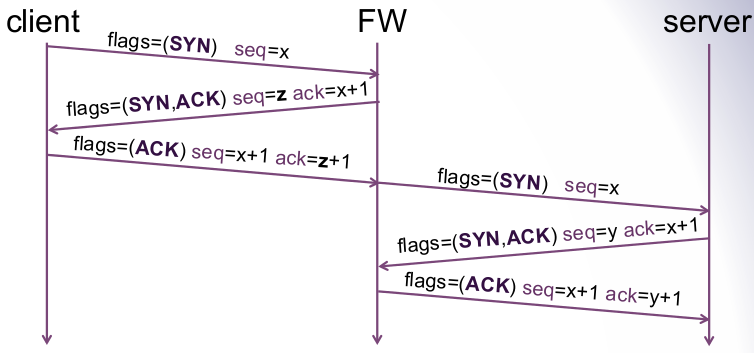
\includegraphics[width=11cm]{img/stateful.png}
\caption{When FW protect SYN flooding, he must adapt all sequence number}
\end{figure}

\subsubsection{Packet Analysis}
Un FW peut analyser les paquets pour vérifier leur format et leur contenu.

\begin{itemize}
  \item Permet l'élimination des paquets malformés (DOS, exploits,...)
  \item Permet l'élimination des paquets qui ne correspondent pas à
l'état actuel du protocole.
  \item Permet d'éliminer des paquets dont le contenu indésirable.
\end{itemize}


\subsection{Proxies}

Un proxy se trouve à la couche application du modèle TCP. 
il est un intermédiaire entre le client et le serveur. Il fait office 
de serveur pour le client et de client pour le serveur. 
Il empêche le réseau interne d'avoir une connexion directe avec Internet.

\begin{figure}[!h]
\centering
\begin{tikzpicture}
\node[draw, rectangle] (A) {Internal Client};
\node[draw, rectangle] (B) [right=4cm of A] {Proxy};
\node[draw, rectangle] (C) [right=4cm of B] {External Server};


\draw (A.east) edge[<->] node[above] {Internal connection} (B.west);
\draw (B.east) edge[<->] node[above] {External connection} (C.west);
\end{tikzpicture}
\caption{Proxy}
\end{figure}


Un serveur proxy permet de réaliser :
\begin{itemize}
  \item Un goulot d'étranglement (chokepoint).
  \item Un accès sur authentification : pour limiter l'accès à Internet
   à un certain nombre d'utilisateur.
  \item Un système de cache : pour avoir un taux de transfert plus rapide 
  et économiser sa bande passante, le proxy va garder une copie locale 
  des documents téléchargés récemment.
  \item Un filtre sur le contenu des paquets : DNS ou URL 
  blacklisté, détection de virus, filtre un mot clé, une URL ou un MIME.
  \item Un reformatage du contenu des paquets : pour transformer une page
   dans le format des PDAs et des Smartphones par exemple.
  \item Faire des tests sur un réseau sans devoir sortir de celui-ci
   (en passant par un proxy situé à l'extérieur).
  \item Permet de surfer anonymement au vu du serveur final mais le
   proxy peut conserver des traces du trafic et donc retrouver la source 
   des requêtes.
   \item Peut augmenter l'efficacité du serveur en utilisant une cache dans le proxy.
\end{itemize}



\subsubsection{Type de proxy}

\paragraph{Proxy Transparent}

Le traffic diriger pour un certain port est automatiquement diriger vers
le proxy. Le proxy ne modifie pas la requête ou la réponse au dela de
ce qui est nécessaire pour l'authentification et l'identification.

\paragraph{Détection}
Il est possible de détecter un proxy transparent par l'adresse IP
(non NATé) ou encore le header http.
\begin{figure}
	\centering
	\begin{tabular}{|c|c|}
	\hline
	\textbf{Avantages}&\textbf{Limitations}\\
	\hline
	Pas besoin de config. browser&Ne fonctionne si port non standard utilisé\\
	Oblige l'utilisation du proxy&\\
	Load Balancing&\\
	\hline
	\end{tabular}
\end{figure}

\paragraph{Reverse HTTP proxy}

Se trouve dans le domaine du serveur et fait du \textbf{load balancing} des
requete entre plusieurs serveurs sans que le client le sâche.

\begin{figure}[!h]
\centering
\begin{tikzpicture}
\node[draw, rectangle] (A) {Internal Client};
\node[draw, rectangle] (B) [right=4cm of A] {Proxy};
\node[draw, rectangle] (C1) [right=4cm of B] {External Server};
\node[draw, rectangle] (C2) [below=of C1] {External Server};
\node[draw, rectangle] (C3) [above=of C1] {External Server};


\draw (A.east) edge[<->] node[above] {Internal connection} (B.west);
\draw (B.east) edge[<->] node[above] {} (C1.west);
\draw (B.east) edge[<->] node[above] {External connection} (C2.west);
\draw (B.east) edge[<->] node[above] {} (C3.west);
\end{tikzpicture}
\caption{Load balancing with reverse Proxy}
\end{figure}

Le client doit d'abord s'authentifier au près du proxy avant de pouvoir
communiquer avec l'un des serveurs.


\subsection{FW avec Zone Démilitarisé}

\begin{figure}[!h]
\centering
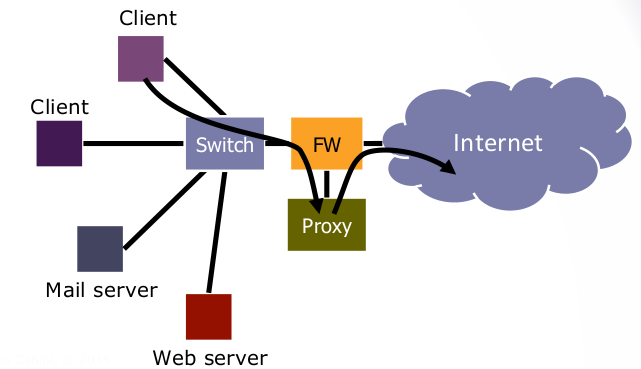
\includegraphics[width=9cm]{img/DMZ.png}
\caption{DMZ}
\end{figure}

La zone démilitarisée (DMZ) n'est relié ni à Internet ni au réseau interne.

\paragraph{Configuration}:
\begin{itemize}
  \item Machines internes peuvent seulement se connecter au proxy.
  \item Seul le proxy peut se connecter à Internet.
  \item Outbound NAT dynamique.
  \item Inbound NAT statique vers le proxy.
  \item Filtrage sortant et filtrage entrant.
\end{itemize}

La limitation de l'exemple (pas de DMZ) est que le firewall est un point
critique et que vu que tout les services par le même proxy, si il y en 
un vulnérable, l'ensemble du traffic devient accéssible. 


\section{Web security}
Dans le temps le web avait une architecture client/serveur tel que 

\begin{itemize}
	\item Le serveur livrait du contenu statique au client.
	\item L'intéraction avec le browser était limité. Le serveur
	était beaucoup plus complexe que le client.
\end{itemize}

La sécurité était donc plus focalisé coté serveur. Maintenant, les 
serveurs peuvent créer du contenu dynamiquement (php,CGI,...) en 
fonction des arguments qu'ils reçoivent (URL par exemple).

\paragraph{Browser}
Les browsers sont devenus plus compliqués. 
\begin{itemize}
	\item Ils peuvent exécuté du code (Javascript par exemple)
	\item Ils peuvent agir comme un support multimédia
	\item Ils peuvent géocaliser l'utilisateur
	\item ...
\end{itemize}

Le web est devenu une plateforme complexe pour le calcul distribué(
ex:Firefox sur windows qui intéragit avec un serveur Linux) ce qui veut
dire que la surface d'attaque est devenu énorme! Dans une application
Web, le contenu provient de plein de site différent. 

La page est découpé en frame:

\begin{figure}[h!]
	\centering
	% Graphic for TeX using PGF
% Title: C:\Users\Nicolas\Pictures\same-origin_frame.dia
% Creator: Dia v0.97.2
% CreationDate: Thu Jun 11 11:17:11 2015
% For: Nicolas
% \usepackage{tikz}
% The following commands are not supported in PSTricks at present
% We define them conditionally, so when they are implemented,
% this pgf file will use them.
\ifx\du\undefined
  \newlength{\du}
\fi
\setlength{\du}{15\unitlength}
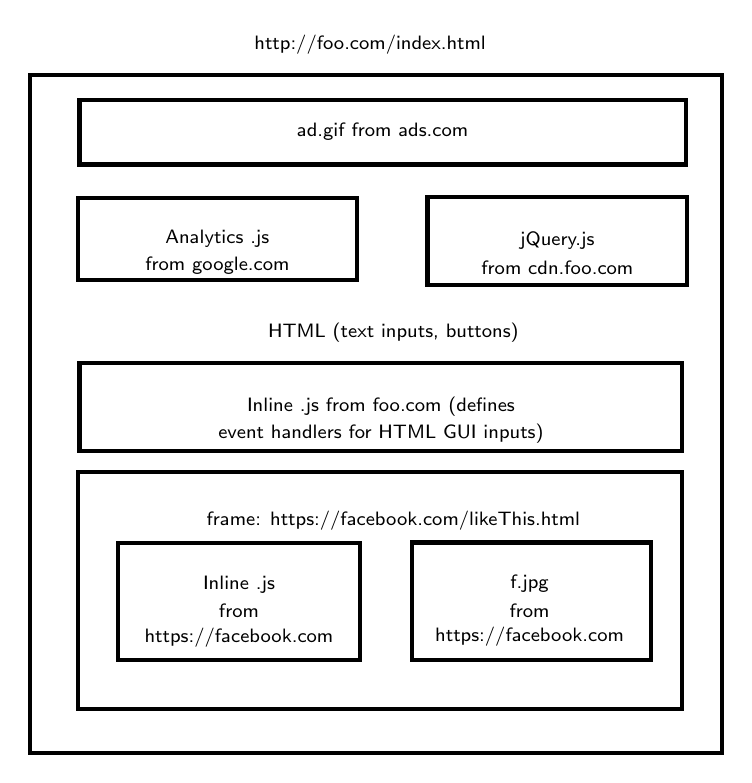
\begin{tikzpicture}
    \scriptsize
\pgftransformxscale{0.800000}
\pgftransformyscale{-0.800000}
\definecolor{dialinecolor}{rgb}{0.000000, 0.000000, 0.000000}
\pgfsetstrokecolor{dialinecolor}
\definecolor{dialinecolor}{rgb}{1.000000, 1.000000, 1.000000}
\pgfsetfillcolor{dialinecolor}
\pgfsetlinewidth{0.100000\du}
\pgfsetdash{}{0pt}
\pgfsetdash{}{0pt}
\pgfsetmiterjoin
\definecolor{dialinecolor}{rgb}{1.000000, 1.000000, 1.000000}
\pgfsetfillcolor{dialinecolor}
\fill (19.950000\du,8.850010\du)--(19.950000\du,29.269405\du)--(40.800000\du,29.269405\du)--(40.800000\du,8.850010\du)--cycle;
\definecolor{dialinecolor}{rgb}{0.000000, 0.000000, 0.000000}
\pgfsetstrokecolor{dialinecolor}
\draw (19.950000\du,8.850010\du)--(19.950000\du,29.269405\du)--(40.800000\du,29.269405\du)--(40.800000\du,8.850010\du)--cycle;
\pgfsetlinewidth{0.100000\du}
\pgfsetdash{}{0pt}
\pgfsetdash{}{0pt}
\pgfsetmiterjoin
\definecolor{dialinecolor}{rgb}{1.000000, 1.000000, 1.000000}
\pgfsetfillcolor{dialinecolor}
\fill (21.450000\du,9.600010\du)--(21.450000\du,11.550000\du)--(39.700000\du,11.550000\du)--(39.700000\du,9.600010\du)--cycle;
\definecolor{dialinecolor}{rgb}{0.000000, 0.000000, 0.000000}
\pgfsetstrokecolor{dialinecolor}
\draw (21.450000\du,9.600010\du)--(21.450000\du,11.550000\du)--(39.700000\du,11.550000\du)--(39.700000\du,9.600010\du)--cycle;
\pgfsetlinewidth{0.100000\du}
\pgfsetdash{}{0pt}
\pgfsetdash{}{0pt}
\pgfsetmiterjoin
\definecolor{dialinecolor}{rgb}{1.000000, 1.000000, 1.000000}
\pgfsetfillcolor{dialinecolor}
\fill (21.400000\du,12.550000\du)--(21.400000\du,15.019405\du)--(29.800000\du,15.019405\du)--(29.800000\du,12.550000\du)--cycle;
\definecolor{dialinecolor}{rgb}{0.000000, 0.000000, 0.000000}
\pgfsetstrokecolor{dialinecolor}
\draw (21.400000\du,12.550000\du)--(21.400000\du,15.019405\du)--(29.800000\du,15.019405\du)--(29.800000\du,12.550000\du)--cycle;
\pgfsetlinewidth{0.100000\du}
\pgfsetdash{}{0pt}
\pgfsetdash{}{0pt}
\pgfsetmiterjoin
\definecolor{dialinecolor}{rgb}{1.000000, 1.000000, 1.000000}
\pgfsetfillcolor{dialinecolor}
\fill (31.925000\du,12.530000\du)--(31.925000\du,15.169405\du)--(39.750000\du,15.169405\du)--(39.750000\du,12.530000\du)--cycle;
\definecolor{dialinecolor}{rgb}{0.000000, 0.000000, 0.000000}
\pgfsetstrokecolor{dialinecolor}
\draw (31.925000\du,12.530000\du)--(31.925000\du,15.169405\du)--(39.750000\du,15.169405\du)--(39.750000\du,12.530000\du)--cycle;
\pgfsetlinewidth{0.100000\du}
\pgfsetdash{}{0pt}
\pgfsetdash{}{0pt}
\pgfsetmiterjoin
\definecolor{dialinecolor}{rgb}{1.000000, 1.000000, 1.000000}
\pgfsetfillcolor{dialinecolor}
\fill (21.450000\du,17.519405\du)--(21.450000\du,20.169405\du)--(39.600000\du,20.169405\du)--(39.600000\du,17.519405\du)--cycle;
\definecolor{dialinecolor}{rgb}{0.000000, 0.000000, 0.000000}
\pgfsetstrokecolor{dialinecolor}
\draw (21.450000\du,17.519405\du)--(21.450000\du,20.169405\du)--(39.600000\du,20.169405\du)--(39.600000\du,17.519405\du)--cycle;
\pgfsetlinewidth{0.100000\du}
\pgfsetdash{}{0pt}
\pgfsetdash{}{0pt}
\pgfsetmiterjoin
\definecolor{dialinecolor}{rgb}{1.000000, 1.000000, 1.000000}
\pgfsetfillcolor{dialinecolor}
\fill (21.400000\du,20.800000\du)--(21.400000\du,27.950010\du)--(39.600000\du,27.950010\du)--(39.600000\du,20.800000\du)--cycle;
\definecolor{dialinecolor}{rgb}{0.000000, 0.000000, 0.000000}
\pgfsetstrokecolor{dialinecolor}
\draw (21.400000\du,20.800000\du)--(21.400000\du,27.950010\du)--(39.600000\du,27.950010\du)--(39.600000\du,20.800000\du)--cycle;
\pgfsetlinewidth{0.100000\du}
\pgfsetdash{}{0pt}
\pgfsetdash{}{0pt}
\pgfsetmiterjoin
\definecolor{dialinecolor}{rgb}{1.000000, 1.000000, 1.000000}
\pgfsetfillcolor{dialinecolor}
\fill (22.600000\du,22.950000\du)--(22.600000\du,26.469405\du)--(29.900000\du,26.469405\du)--(29.900000\du,22.950000\du)--cycle;
\definecolor{dialinecolor}{rgb}{0.000000, 0.000000, 0.000000}
\pgfsetstrokecolor{dialinecolor}
\draw (22.600000\du,22.950000\du)--(22.600000\du,26.469405\du)--(29.900000\du,26.469405\du)--(29.900000\du,22.950000\du)--cycle;
\pgfsetlinewidth{0.100000\du}
\pgfsetdash{}{0pt}
\pgfsetdash{}{0pt}
\pgfsetmiterjoin
\definecolor{dialinecolor}{rgb}{1.000000, 1.000000, 1.000000}
\pgfsetfillcolor{dialinecolor}
\fill (31.450000\du,22.930000\du)--(31.450000\du,26.469405\du)--(38.650000\du,26.469405\du)--(38.650000\du,22.930000\du)--cycle;
\definecolor{dialinecolor}{rgb}{0.000000, 0.000000, 0.000000}
\pgfsetstrokecolor{dialinecolor}
\draw (31.450000\du,22.930000\du)--(31.450000\du,26.469405\du)--(38.650000\du,26.469405\du)--(38.650000\du,22.930000\du)--cycle;
% setfont left to latex
\definecolor{dialinecolor}{rgb}{0.000000, 0.000000, 0.000000}
\pgfsetstrokecolor{dialinecolor}
\node at (30.575000\du,10.575005\du){ad.gif from ads.com};
% setfont left to latex
\definecolor{dialinecolor}{rgb}{0.000000, 0.000000, 0.000000}
\pgfsetstrokecolor{dialinecolor}
\node at (25.600000\du,13.784702\du){Analytics .js };
% setfont left to latex
\definecolor{dialinecolor}{rgb}{0.000000, 0.000000, 0.000000}
\pgfsetstrokecolor{dialinecolor}
\node at (25.600000\du,14.584702\du){from google.com};
% setfont left to latex
\definecolor{dialinecolor}{rgb}{0.000000, 0.000000, 0.000000}
\pgfsetstrokecolor{dialinecolor}
\node[anchor=west] at (25.600000\du,13.784702\du){};
% setfont left to latex
\definecolor{dialinecolor}{rgb}{0.000000, 0.000000, 0.000000}
\pgfsetstrokecolor{dialinecolor}
\node at (35.837500\du,13.849702\du){jQuery.js };
% setfont left to latex
\definecolor{dialinecolor}{rgb}{0.000000, 0.000000, 0.000000}
\pgfsetstrokecolor{dialinecolor}
\node at (35.837500\du,14.649702\du){ from cdn.foo.com};
% setfont left to latex
\definecolor{dialinecolor}{rgb}{0.000000, 0.000000, 0.000000}
\pgfsetstrokecolor{dialinecolor}
\node[anchor=west] at (30.375000\du,19.059707\du){};
% setfont left to latex
\definecolor{dialinecolor}{rgb}{0.000000, 0.000000, 0.000000}
\pgfsetstrokecolor{dialinecolor}
\node at (30.900000\du,16.625000\du){HTML (text inputs, buttons)};
% setfont left to latex
\definecolor{dialinecolor}{rgb}{0.000000, 0.000000, 0.000000}
\pgfsetstrokecolor{dialinecolor}
\node at (30.525000\du,18.844405\du){Inline .js from foo.com (defines};
% setfont left to latex
\definecolor{dialinecolor}{rgb}{0.000000, 0.000000, 0.000000}
\pgfsetstrokecolor{dialinecolor}
\node at (30.525000\du,19.644405\du){ event handlers for HTML GUI inputs)};
% setfont left to latex
\definecolor{dialinecolor}{rgb}{0.000000, 0.000000, 0.000000}
\pgfsetstrokecolor{dialinecolor}
\node at (30.900000\du,22.270005\du){frame: https://facebook.com/likeThis.html};
% setfont left to latex
\definecolor{dialinecolor}{rgb}{0.000000, 0.000000, 0.000000}
\pgfsetstrokecolor{dialinecolor}
\node at (26.250000\du,24.200005\du){Inline .js };
% setfont left to latex
\definecolor{dialinecolor}{rgb}{0.000000, 0.000000, 0.000000}
\pgfsetstrokecolor{dialinecolor}
\node at (26.250000\du,25.000005\du){from };
% setfont left to latex
\definecolor{dialinecolor}{rgb}{0.000000, 0.000000, 0.000000}
\pgfsetstrokecolor{dialinecolor}
\node at (26.250000\du,25.800005\du){https://facebook.com};
% setfont left to latex
\definecolor{dialinecolor}{rgb}{0.000000, 0.000000, 0.000000}
\pgfsetstrokecolor{dialinecolor}
\node at (35.000000\du,24.175005\du){f.jpg};
% setfont left to latex
\definecolor{dialinecolor}{rgb}{0.000000, 0.000000, 0.000000}
\pgfsetstrokecolor{dialinecolor}
\node at (35.000000\du,24.975005\du){ from};
% setfont left to latex
\definecolor{dialinecolor}{rgb}{0.000000, 0.000000, 0.000000}
\pgfsetstrokecolor{dialinecolor}
\node at (35.000000\du,25.775005\du){ https://facebook.com};
% setfont left to latex
\definecolor{dialinecolor}{rgb}{0.000000, 0.000000, 0.000000}
\pgfsetstrokecolor{dialinecolor}
\node at (30.200000\du,7.927073\du){http://foo.com/index.html};
\end{tikzpicture}

\end{figure}
$\to$ La question est quelle partie de JS peut accéder à quoi?

\subsection{Same-origin policy}

Pour répondre à cette question, les browsers utilisent un modèle de
sécurité appelé \textbf{Same-origin policy}. L'idée est que deux
sites différents ne devrait pas pouvoir altérer le contenu entre eux.

\begin{itemize}
	\item Le browser assigne une origine à toute les ressources de
	la page (librarie javascript,images,...).
	\item Le code JS ne peut accéder que les ressources provenant de la 
	même origine.
\end{itemize}

\paragraph{Origin}
Une origine a la forme : \texttt{protocole + nom de l'hôte + port}. 
(Protocole peut être http,https,ftp,file,\ldots)

Il y a 4 idées principales:
\begin{itemize}
	\item Une origine est associé avec une ressource coté client. (Une 
	origine est l'équivalent moral d'un UID en Unix)
	\item Chaque frame de la page prend l'origine de son URL. (Une 
	frame est l'équivalent moral d'un proccess en Unix)
	\item Les scripts inclus par les frame s'execute avec l'autorité 
	de l'origin du fichier HTML. Vrai pour pour les scrips ''maison''
	et ceux de domain externes. (Analogie :Executer le binaire qui est
	stocké dans le repertoire home de quelqu'un d'autre.)
	\item Le contenu passif n'a aucune autorité puisqu'il ne peut 
	pas executer de code.
\end{itemize}
Dans l''exemple, le code JS dans frame de facebook n'a pas accès aux 
ressources dans la frame foo.com.

\subsubsection{Browsers}

\paragraph{Frame}

Un object frame est un DOM (Document Object Model: description d'une 
interface indépendante de tout langage de prog. et de la platetforme). 

Pour récupérer l'origine d'un frame:
\begin{itemize}
	\item Récupérer l'origine via l'URL de la frame
	\item[OU]
	\item Récupérer l'origine via le document (document.domain).
	document.domain est à la base dérivé de l'URL et ensuite peut être changé.
	Il peut contenir un suffix du domain complet (z.com au lieu de x.y.z.com) 
\end{itemize}

$\to$ Les browser séparent document.domain changé et ceux inchangé (même si
ils ont le même document.domain). 

Deux frames peuvent s'accéder mutuellement si ils ont le même document.domain

\paragraph{DOM}
Prenne l'origine de la frame environnante

\paragraph{Cookies}
Un cookie est composé d'un domaine et d'un chemin (ex: *.mit.edu/6.858/).
Le code JS peut avoir accès à n'importe quel cookie qui correspond à 
l'origine du code (attention chemin et port d'origine sont ignoré dans
compaison). 

\subsubsection{Exeception Modèle}
Ils existent quelques execeptions au modèle:
\begin{itemize}
	\item De base, JS peut seulement envoyer des XMLHttpRequest à son 
	serveur d'origine sauf si un autre serveurs active le 
	\textbf{Cross-Origin Resource Sharing} (CORS).
	\item A frame peut charger une image de n'importe quelle origine,
	determiner la taille mais ne peut pas regarder les pixels dedans.
	\item Une frame peut chargé un JS de n'importe quelle origine mais
	elle ne peut pas directement examiner le code source.
	\item Une frame peut executer un plugin de n'importe quelle origine 
\end{itemize}
%TODO CSRF

\subsubsection{Réseau}
Une frame peut envoyer une requête HTTP et HTTPS au hôte+port
qui correspondent à son origine.
$\to$ La sécurité de la same-origin policy dépend de l'intégrité 
l'infrastructure DNS! (le mapping entre l'hôte et l'ip doit être correct) %Example DNS?

\subsubsection{Pixels}
Les pixels n'ont pas d'origine, une frame peut dessiner où elle veut dans
ses limites. Cela veut dire qu'une frame parent peut cacher le contenu
d'une frame enfant. Solution:
\begin{itemize}
	\item Inclure JS qui empêche la page d'être inclus comme frame.
	\item Ajouter l'en-tête X-Frame-Options dans la réponse 
	pour dire au browser de ne placer le contenu dans une frame enfant
\end{itemize}
\subsubsection{Frame sans Origin}
On peut avoir frame du style : file://foo.txt, cette frame n'a pas
d'origin. Différent scénario possibles:
\begin{itemize}
	\item La frame est accessible pour les frames avec le même protocole. 
	(file://)
	\item La frame est inaccessible pour toutes les autres origine.
	\item La frame hérite de l'origine de ce qui a créé la frame.
\end{itemize}
\subsection{HTML5}
HTML 5 apporte une API de partage d'écran. Si l'utilisateur
donne l'autorisation, un site peut capturer l'entièreté de l'écran visible et 
se transmettre la capture.
$\to$ Si un attacker parvient à convaincre un utilisateur à 
utiliser cette sur un de ses sites, il peut réussir à récupéter les cookies.

\subsection{Conclusion}
 Modèle de sécurité de browser c' est un peu le foutoir. Il y a beaucoup
 de subtilité et d'inconsistence. Le réecrire apporterait pas mal de 
 problème:
 \begin{itemize}
	\item Beaucoup d'infrastrucute web préexistante sur lesquelles
	les gens comptes.
	\item Moins de features pour plus de sécurité?
	\item...
\end{itemize}

\section{Web Attack and Defense}

\subsection{Shell Shock code}
Un serveur Unix map les composants d'une requête HTTP(extra headers) dans des variables 
d'environments. 

\paragraph{Problème}
Le probleme est que bash a un bug dans son parsing. Si un string commence
avec un ensemble de bytes mal formé, bash continue le parsing et execute 
les commande qu'ils trouvent.

\subsection{XSS defenses}

\paragraph{XSS}
C'est un bonne exemple de mauvaise désinfection de contenu. Une 
attaque XSS consiste à injecter du code (ex:JS) dans une page coté 
client qui sera ensuite vu par d'autre client. Á ce moment là,
le browser exécutera le code. 


\subsubsection{Heuristiques}
Les browsers modernes utilisent une heuristique pour detecter les
attaques XSS. 
\begin{itemize}
	\item Est-ce que le script qui veut s'executer est inclus dans la 
	requête (l'URL)qui a amener l' 'enclosing page'' ? Si oui,
	alors c'est une attaque%an enclosing page?
	\item Efficace contre les attaques reflechies (réfléchies car 
	serveur renvoie le code de l'attacker au browser de l'utilisateur)
	 %Je suis même pas sur que la trad est correct
\end{itemize}
Cette technique ne fonctionne pour les attaques XSS persistente 
(ex: code dans une section commentaire)

\subsubsection{Type}

\begin{enumerate}

\item \textbf{Set-Cookie: Httponly}
Une façon de se défendre est d'utiliser les Httponly cookie. Le serveur
dit au browser que le JS coté client ne peut pas avoir accés au cookie.

$\to$ Pas assez puissant car l'attacker peut toujours faire des requêtes
avec le cookie de l'utilisateur. (CSRF)

\item \textbf{Séparation de Privilièges}
Utiliser un domain séparé pour le contenu dans lequel on a pas confiance
(C'est ce Google fait). Si jamais l'attaque est possible, le code tourne dans 
un autre domaine.

$\to$ Devient un problème si le contenu du domaine séparé pointe vers 
le domaine principale.

\item \textbf{Désinfection du contenu}
L'idée est de prendre le contenu dans lequels on a pas confiance et de
l'encoder de façon à limiter la façon dont il peut être interpréter.

$\to$ Il difficile de parser l'HTML de façon non-ambigüe.

\paragraph{Alternative}
Une autre façon de faire serait d'interdire l'HTML venant de l'extérieur
et forcer ce contenu extérieur à être écrit dans un plus petit langage.
(Ce langage sera alors traduit en HTML).

\item \textbf{Content Security Policy}
Les serveurs web informent les browsers de quels types de ressources
peuvent être chargées et les origines autorisées pour ces ressources.

\end{enumerate}


\subsection{Session management}

La solution classique consiste à mettre une random session ID
dans le cookies.

Les sessions expirent après un certain délai.

\subsubsection{Stateless Cookies}

Si la notion de session disparait, il faut un moyen pour authentifier 
chaque requêtes. L'idée est d'authentifier les cookie en utililsant la 
crypto (MAC).

\paragraph{Fonctionnement}
Le client et le serveur se partage un clé qui va être utiliser pour 
envoyer (coté client) et vérifier les messages (coté serveur).  

\paragraph{Alternative}
Ils existent des alternatives aux cookies pour la gestion de session
\begin{itemize}
	\item Utiliser le stokage local de HTML5 et implémenter 
	l'authentification en JS. Cela a l'avantage 
	de ne pas devoir envoyer le cookie via le network et ce 
	n'est pas sujet au modèle complexe de same-origin policy.

	\item Certificat coté client %TODO
\end{itemize}

\subsection{Ambiguité des protocols}
\begin{itemize}
	\item JS peut demander au browser d'envoyer une XMLHttpRequest et
	d'ajouter des en-tête à la requêtes. Le problème c'est que les valeurs 
	de ces en-tête peut être en conflict avec celle calculé par le browser.
	(Content-length,Host,...)	

	\item Le parsing d'une URL peut amené de l'ambiguité: http://example.com:80@foo.com/
	\begin{itemize}
		\item Pour Flash l'origine est example.com
		\item Pour le browser c'est foo.com
	\end{itemize}
\end{itemize}


\section{Systèmes de détection d'intrusion (IDS)}

Les IDS analysent le trafic réseau (réseau IDS, NIDS), généralement
en face du pare-feu et/ou les événements sur les serveurs (Host IDS, HIDS).

\textbf{En cas d'attaque}, ils lancer une alarme (SMS, courrier,
etc) et permettent de reconfigurer le pare-feu (filtrage de l'attaque)
ou les serveurs.

L'analyse peut se faire en temps réel ou en analysant les logs.

\subsection{Réaction au attaque}
Systèmes de prévention des intrusions (IPS):
    Un IPS est un IDS qui réagit à une attaque.
    \begin{itemize}
    \item Niveau IP: Filtres l'adresse IP source dans le pare-feu (pour un temps).
    \item Niveau TCP: Envoie un spoofed paquet TCP 'reset' à la destination pour tuer la connexion.
    \item Niveau application: «corrige» une requête Web pour enlever les caractères spéciaux.
    \end{itemize}

\subsection{Type}

\begin{enumerate}
\item IDS avec caractérisation du trafic (IDS with Traffic Characterization):
    réalise des statistiques sur le trafic.

    $\to$ Si la valeur va au-delà de ses limites habituelles, alors
        l'IDS suppose qu'il y a une attaque.

    \begin{itemize}
        \item Peut reconnaître de nouvelles attaques.
        \item faux négatifs
        \item faux positifs (taux élevé)
    \end{itemize}

\item IDS basés sur les signatures (Signature-based IDS):
    dispose d'une base de données avec les attaques connues.

    \paragraph{Attention} Il ne reconnaît pas de nouvelles attaques
(besoin de màj). Les faux négatifs.

    \begin{itemize}
    \item Attaques manuelles peuvent avoir des variations qui ne sont pas détectés.
    \item Les signatures sont pas toujours précis. (Les faux positifs)
    \item L'IDS, dans la plus part des cas, ne sait pas si une tentative d'attaque a réussi.
    \item L'IDS ne sait pas si la cible de l'attaque est vulnérable (par exemple attaque Linux sur serveur
            Windows).
    \end{itemize}
    Exemple d'IDS basés sur les signatures : Snort

\item IDS basé sur l'intégrité de l'host (Integrity-based Host IDS):
    Tripwire est un exemple typique d'un HIDS avec une analyse différée.
    \begin{itemize}
    \item Il crée une signature numérique de tous les fichiers et répertoires qui ne doivent pas être
    modifiés.
    \item Les signatures ne peuvent pas être modifiées par un pirate.
    \item Il compare régulièrement les fichiers et les signatures pour détecter d'éventuelles
    modifications.
    \item Il génère une alarme lorsqu'il détecte une modification et peut restaurer automatiquement la
    version originale du fichier.
    \end{itemize}
\end{enumerate}


\section{Certificates}

\subsection{Bases}

L'objectif d'un certificat est de relier une clé publique avec son propriétaire.

\begin{itemize}
	\item Le couple (clé publique, propriétaire) est signé par un tiers de 
	confiance appelé autorité de certification (CA). Pour vérifier la signature
	, la clé publique de le CA est nécessaire.
	\item Le couple (clé publique du CA, CA) est auto-signé: certificat 
	racine. L'authenticité du certificat racine est fondamentale.
\end{itemize}

\paragraph{Trois champs obligatoires}

\begin{itemize}
  \item \textbf{TBS certificat} (TBS = " To Be Signed "): La charge utile du certificat, elle contient
  	\begin{itemize}
		\item Numéro de série: Numéro unique attribué par le CA à la certificat.
  		\item Domaine de la société: Identifies l'entité qui a signé et délivré le certificat.
 		\item Sujet: Identifies l'entité associée à la clé publique 
 		(O: organisation, C: pays, OU: Unité d'oranisation, CN: nom commun 
 		par exemple DNS, ST:  Etat, L: ville, etc Aucune adresse IP).
 		\item Validité: Pas avant, pas après.
		\item Subject Public Key Info: La clé publique et identification de 
		l'algorithme avec lequel la clé est utilisée.
	\end{itemize}
  \item \textbf{CA algorithme de signature}: identificateur de l'algorithme 
  cryptographique utilisé par l'AC pour signer le certificat.
  \item \textbf{Valeur de signature CA}: Signature du certificat par le CA.
\end{itemize}

\subsection{Obtenir et vérifier un certificat}

Le couple (clé publique du CA, CA) est auto-signécertificat racine.
L'authenticité du certificat racine est fondamentale.

\paragraph{Etapes}
\begin{enumerate}
	\item Le postulant s'enregistre avec un CA.
	\item Le CA (physiquement) authentifie le demandeur.
	\item Le CA demande au participant de générer des clés publiques / privées.
	\item Le CA crée un certificat avec l'identité du demandeur, la clé 
	publique, la date d'expiration, etc,et la signature du CA.
	\item Le CA fournit une copie de sa clé publique à la postulant.
	\item Le demandeur peut propager son certificat.
\end{enumerate}

$\Rightarrow$ Un CA peut décider déléguer l'enregistrement d'un postulant à une 
autorité d'enregistrement (RA). Le RA remplit juste un requête de 
signature de certificat (CSR) pour que le CA remplit le certificat.

\paragraph{Vérification d'un certificat}
\begin{itemize}
  \item Vérifiez le chemin de certification.
  \item Vérifiez la période de validité.
  \item Vérifiez que le certificat n'est pas révoqué.
\end{itemize}

\paragraph{Note:} Même si un certificat compromis est revoqué et
remplacé par un nouveau, un site sécurisé peut toujours être 
vulnérable.

\subsection{SSL/TLS}

SSL inventé à la base pour offrir un protection de la communication en
se focalisant sur la couche transport (SSL entre la couche transport et
Application). \\

Plusieurs version de SSL existent, le version est celle qui a amené à TLS.
Par défaut, les protocols comme SMTP ou HTTP envoie les mots de passes
en texte clair. TLS permet de palier à se problème en étendant ces protocoles

\subsection{TLS protocole}
\begin{figure}[h]
	\centering
	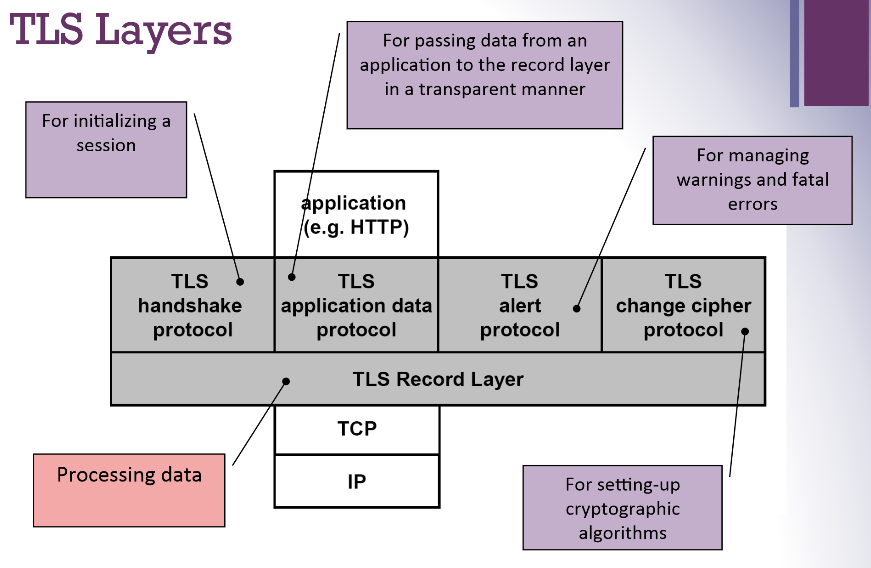
\includegraphics[scale=0.5]{img/tls_layer.png}
\end{figure}
TLS comprend 4 protocoles et deux couches:
\begin{description}
	\item[TLS Record Layer] Couche la plus basse, elle applique aux 
	données les protocoles cryptographiques négociés. Elle se charge 
	de la compression/fragmentation des données. Transmet les données
	à la couche TCP.
	\item[Couche plus haute] comporte 4 protocoles
	\begin{itemize}
		\item \textbf{Handshake Protocol} : Il est utilisé pour authentifier les deux
		entités et négocier les algorithmes de chiffrement et 
		d'authentification.
		\item \textbf{Application Protocol} : transmet les données entre l'
		application et la couche basse de TLS.
		\item \textbf{Alert Protocol} : est utilisé pour informer 
		l'application sur l'état de la connexion. (ex: Certificat invalide)
		\item \textbf{Change Cipher Protocol}: informe l'application qu'un 
		ensemble de protocoles cryptogaphiques précédemment négocié 
		va être utilisé.
	\end{itemize}
\end{description}
\subsection{TLS Record Layer}
\paragraph{MAC Computation}
$$MAC = Hash(MAC\_key || Pad2 || Hash ( MAC\_Key || Pad1 || Seq || Length
	|| Content))$$ Où :
\begin{itemize}
	\item MAC\_key : clé secrète partagée par les 2 entitées
	\item Pad1,Pad2 : constantes prédéfinies
	\item Seq: n° de séquence de message
	\item Length: Longueur en byte du record compressé
	\item Content : record compressé
\end{itemize}
\paragraph{Encryption}
Utilisation d'un chiffrement en bloc (DES,AES,...) ou en Stream (NULL,RC4)
Attention si le serveur propose un d'utiliser RC4 avec une clé de 40-bits $\to$ REFUSE.
\subsection{Handshake}
Les messages lors de l'handshake ne sont pas cryptés, les entitées négocient:
\begin{itemize}
	\item La version du protocole (SSL 3.0,TLS 1.0,1.1)
	\item Algo pour:
	\begin{itemize}
		\item Échanger les clés (RSA,Diffe-Hellman)
		\item Encrypter (3DES,AES,...)
		\item MAC (HMAC-MD5,HMAC-SHA)
	\end{itemize}
\end{itemize}
Le client propose les algo désirés par ordre de préférence et le serveur
choisis.
\begin{figure}[h]
	\centering
	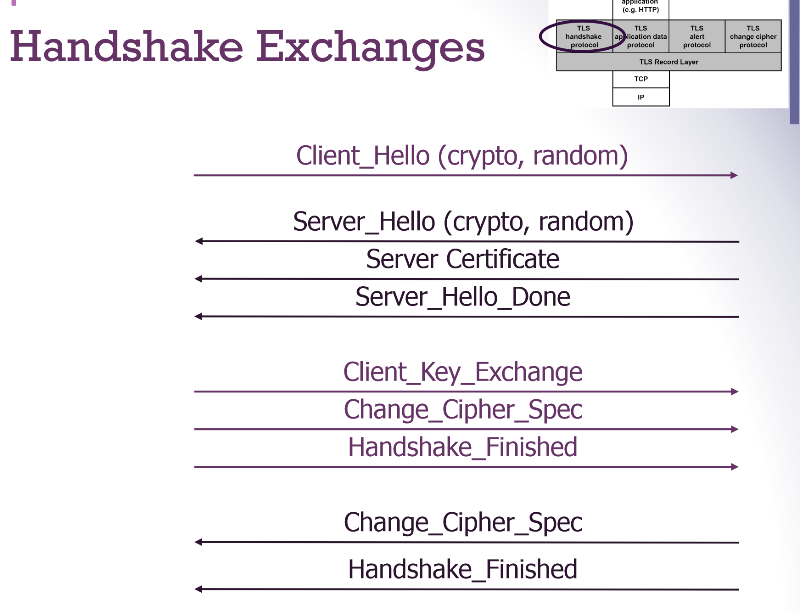
\includegraphics[scale=0.5]{img/handshake.png}
\end{figure}
\paragraph{Pretty Good Privacy}
Ce fut le premier logiciel qui permettait de protéger les documents
et les messages. Il utilisait les algo de cryptographie tel que 
RSA,SHA-1,...

\section{Passwords}
\subsection{Stockage}
Les mot de passe ne doivent jamais être stocké en clair.
\begin{itemize}
	\item Á la place de stocker le password, stocké une valeur de hash.
	Il faut pour cela que la valeur de hash soit irreversible.
	\item Pour le login, hashé le mot de passe et ensuite comparer avec
	la valeur stocké.
\end{itemize}
\subsection{Vulnerabilités}
Quelques vulnérabilités :
\begin{itemize}
	\item Noter un mot de passe:
	\item Les regards indiscrets
	\item Ingénierie sociale (ex: envoyer un mail qui demande la
	confirmation d'un mot de passe en envoyant le mot de passe)
	\item Key Loggers
	\item Écoute du réseau
	\item Multi-Website Password 
	\item Les traces (ex: gestionnaire de mot de passe (qui les enregistre)
	sur les ordinateurs public.
	\item Attaques par essaie erreurs 
\end{itemize}

\subsection{Online attack}
Les online attack consistent à tester des mots de passe successivement à travers l'interface (web par
exemple) qui sépare le pirate et le serveur.\\
Le serveur va alors indiquer au pirate si le mot de passe est
bon ou non et dans ce cas, essayer un autre (le serveur fonctionne comme une black box, un oracle).
Ce système est lent, mais ne nécessite pas de connaitre la fonction de hash.
Pour contrer ce genre d'attaque :
\begin{itemize}
  \item Ajouter un délai de réponse :Un délai est ajouté avant que le client (pirate ici) ne reçoit la
réponse du serveur.
  \item Notifier l'utilisateur (par mail) et bloquer son compte : Attention, cette mesure permet de faire
du déni de service. En effet, un pirate peut essayer plusieurs mot de passe random pour
bloquer le compte d'un utilisateur. L'utilisateur va alors contacter le service client et cela aura
également un coup pour celui-ci.
  \item Faire participer l'utilisateur : La machine du client doit faire un grand nombre d'opération
avant de pouvoir soumettre un mot de passe (trouver un « r » tell que h(login,password,r)
renvoie un nombre dont les derniers bits soit égaux à 0). Cela ralentit considérablement la
vitesse des attaques tout en maintenant un temps de calcule raisonnable pour une simple
connexion.
  \item Captcha : La plupart des attaques se font par des ordinateurs alors que la vraie connexion par
des humains. Il suffit donc de demander au client une réflexion simple pour un humain mais
compliqué pour un ordinateur.
\end{itemize}
\subsection{Offline attack}
Les offline attack consiste à voler le fichier qui contient tous les hash, trouver la fonction de hash et
ensuite faire une attaque par dictionnaire, brute force, etc. En connaissant la fonction de hash, le
pirate peut comparer des mots de passe hashé au fichier récupérer sur le serveur.
\subsection{Attaques par dictionnaire}
Beaucoup de gens utilise des mots de passe issus du dictionnaire (plus simple à retenir) mais celui-ci
est fini (entre 150000 mots et 200000 mots) et est réduit donc considérément les possibilités. Un
dictionnaire déjà hashé peut accélérer l'attaque. Un ordinateur peut calculer entre 200 000 hash et 10
000 000 hash par second en fonction de la fonction de hash.
\subsection{Brute-force}
Les attaques par brute-force consiste à essayer un grand nombre de possibilité même si celle-ci n'ont
pas obligatoirement un sens (« aaa » puis « bbb » puis « abb », etc). Cette attaque permet de trouver
les mots de passe abstrait sans signification qui ne se trouve pas dans un dictionnaire.
\paragraph{Heuristique d'attaque}
On peut combiner l'attaque par dictionnaire et l'attaque par brute force en appliquant certaines règles
souvent utilisé par les gens :
\begin{itemize}
  \item Convertir majuscule/minuscule (FRED/fred).
  \item Mettre la première lettre en majuscule (Fred).
  \item Inverser les lettres d'un mot (Derf).
  \item Dupliquer un mot (FredFred).
  \item Réfléchir un mot (Fredderf).
  \item Décaler les lettres vers la gauche ou la droite (Redf/Dfre).
  \item Remplacer certain caractère par des similaires (Fred).
  \item Ajouter X caractère au début ou à la fin du mot (aaaFred).
\end{itemize}
\subsection{Faiblesse}
Les mots de passes considéré comme faibles sont ceux:
\begin{itemize}
	\item basé sur des mots communs du dictionnaire
	\item basé sur des noms communs
	\item qui ont moins de sept caractères
	\item basé sur les pattern du clavier (''qwerty''...)
	\item composé d'un seul type de symbole 
\end{itemize}
\subsection{Authentification Unix}
La fonction de hash peut être basé sur le DES, MD5, Blowfish, SHA256, SHA512.
\subsubsection{Unix (DES)}
Le méchanisme consiste à générer la hash d'un mot de passe en chiffrant
25 fois avec une variante de l'algorithme DES une chaîne de caractère null 
(64bit valant 0).\\
La clé de chiffrement est le mot de passe à hacher. On
ne prend que le 8 premiers charactère du mots de passe et on 
extrait les 7bits de poids faible de chaque caractères $\to$ clé de
56 bits pour le DES.\\
L'algo utilise en plus un paramètre de 12 bits appelé \textbf{salt} 
(générer aléatoirement à la création du mit de passe).
Il permet que deux utilisateurs ayant le même mots de passe n'est
pas le même valeur de hash.
\begin{figure}
	\centering
	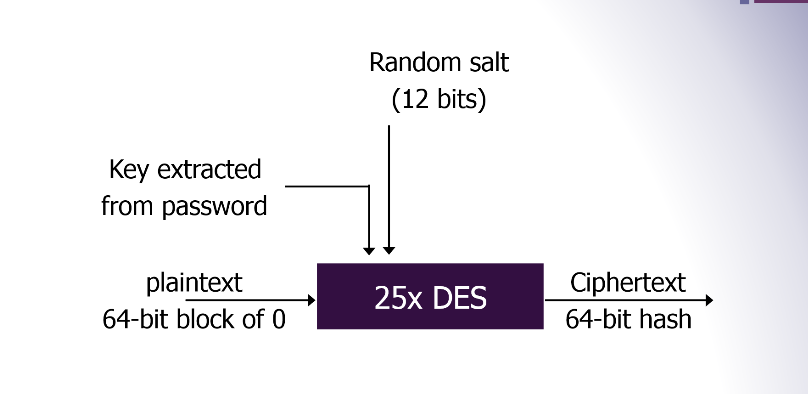
\includegraphics[scale = 0.5]{img/auth_unix_des.png}
\end{figure}

Le hash est stocké dans le fichier /etc/shadow sous la forme :
$$username:passwd:last:may:must warn:expire:disable:reserved$$
Où :
\begin{itemize}
	\item passwd est le salt la valeur de hash
	\item last/may/must/... sont de champs qui contients
	des infos temporelle sur le mot de passe, tel que 
	le nombre de jours avant qu'il puisse (may) ou doit (must) être modifié.
\end{itemize}
\subsubsection{Unix(MD5)}
Le DES devenu obsolète, une alternative est MD5. Comparé un DES qui est
un algorithme de chiffrement, MD5 est un fonction de hachage.\\
MD5 permet l'utilisation des mot de passes plus longs et les charactères
ne sont plus limités à 7 bits.\\
Le salt n'est plus sur 12 bits mais 48 bits (8 caractère encodé en 
Base64).\\
La valeur de hash est sur 128 bits.
\begin{figure}[h]
	\centering
	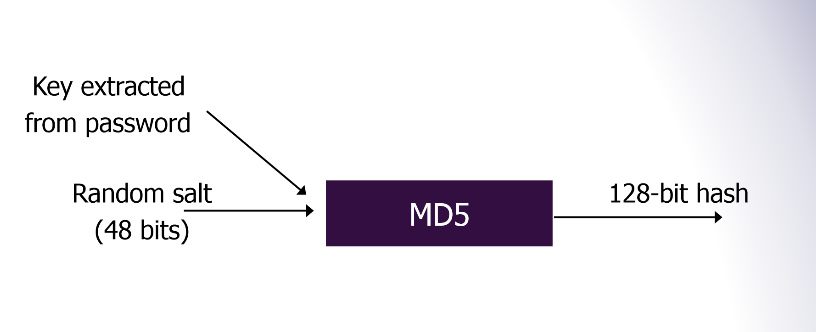
\includegraphics[scale = 0.5]{img/auth_unix_md5.png}
\end{figure}
Dans le fichier /etc/shadow, le champs passwd commence avec \$1\$ pour
indiquer l'utilisation de MD5.Le salt est ensuite concaténé et se termine 
par \$. Ensuite viens la valeur de hash.
\subsection{Authentification Windows}
\subsubsection{Win9x}
Windows utilise le Lan Manager Hash pour hasher ses mots de passe.
Le mot de passe est d'abord converti en majuscule puis divisé en deux 
blocks de 7 caractères après l'avoir complétés avec le char vide pour qu'il 
atteingne 14 caractères \\
Chaque bloc de 7 bytes est utilisé comme clé pour crypter une constante
avec l'algorithme DES (pas d'utilisation de salt). Il y a donc 2 valeur 
de hash de 64bits qui sont ensuite concaténé.
%%TODO faire un belle image
\subsubsection{Win NT/2000/XP/Vista/Seven}
Ces versions de Windows utilisent le NT Lan Manager Hash (NT Hash) qui 
utilise MD4.\\
Cette fois, le mot de passe n'est pas:
\begin{itemize}
	\item pas séparé en deux 
	\item peut-être plus grand que 14 caractères
	\item et n'est pas converti en majuscule.
\end{itemize}
\subsubsection{Stockage des mots de passe }
Par défaut, LM Hash et NT Hash sont tous les deux conservés sur la 
machine (jusqu'à Windows XP compris). Il est donc possible de récupérer 
le mot de passe NT Hash en récupérant le mot de passe LM
Hash. \\
Il est possible de désactivé le LM Hash (désactivé par défaut à partir de
Vista), dans le registre ou en choisissant un mot de passe de plus de 14 
caractères.
En dessous de W2K, XP et 2003, NT Hash et LN Hash sont stockés dans le 
Security Account Manager ou dans le Active Directory (ntds.dit).\\
Le fichier est crypté mais par défaut la clé est récupérable et le
fichier de hash également avec les droits administrateur et un exploit 
ou en bootant sur un autre OS.
\subsection{Bonnes pratiques}
Un mot de passe doit contenir au moins un élément de chaque point 
\begin{itemize}
	\item Digit (0..9)
	\item Letter (a..Z)
	\item Ponctuation (?!)
	\item Caractère de controle (Ctrl+s, $^s$)
	\item Un caractère spécial dans les 7 premiers caractère (pourquoi 7 ?)
\end{itemize}
Ne pas recyclé de mot de passe ou noter ses mots de passe.
Utiliser des niveaux de sécurité.
Modifier son mot de passe immédiatement si on pense avoir été victime d'une attaque.
Ne pas utiliser l'option « retenir mon mot de passe ».

\section{Time-memory Trade-off}
\subsection{Motivations}
\paragraph{One-Way function (hash function)}
Une fonction $h:\ A\to B \ $ qui est facile à calculer pour tout les 
input, mais qui est difficiler à inversé pour une image d'un input 
aléatoire.\\

\paragraph{Exaustive search :}
- Recherche en temps réel (online) : recherche (N = \#(A)) stockage (0) pré-calcule (0)
- Recherche pré-calculé (offline): recherche (0) stockage (N) pré-calcule (N)

\subsection{Hellman Tables}
Les table de Hellman est un principe de pré-calcul qui améliore considérablement la vitesse d'une
attaque en temps réelle.

\subsubsection{Création d'une table}
Soit,
\begin{description}
\item[H]: A $\to$B La fonction de hashage de notre mot de passe.
\item[R]: B $\to$ A Une fonction (arbitraire, rapide, surjective, déterministe) de réduction qui permet de
revenir à l'ensemble (A) de départ de notre fonction de hashage.
\end{description}
Un nombre M de chaine est généré avec comme départ une valeur arbitraire de départ dans A :
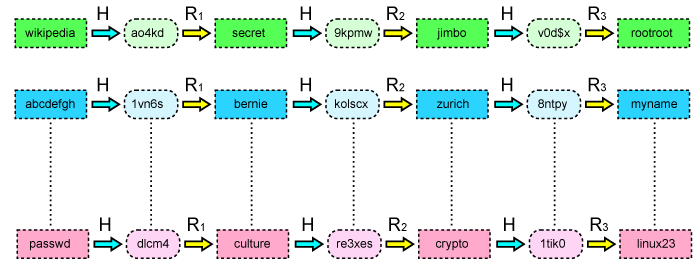
\includegraphics[width=15cm]{img/rainbow.png}


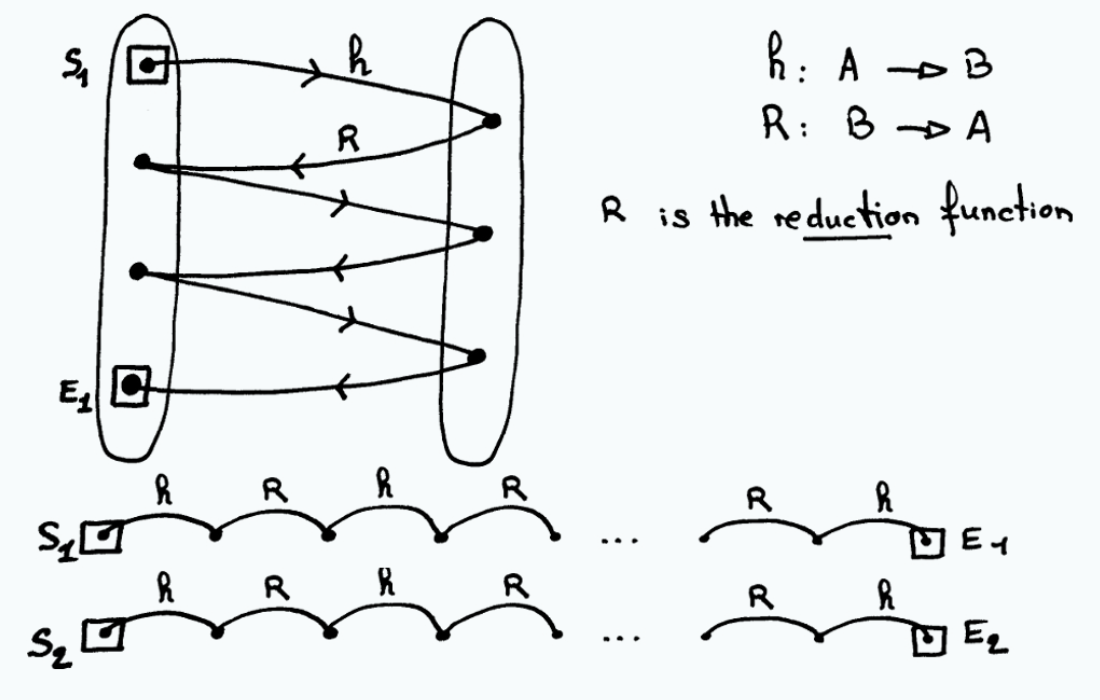
\includegraphics[width=15cm]{img/rain2}

A la fin du pré-calcule d'une chaine, on ne garde que la première valeur et la dernière valeur de la chaine. Les valeurs intermédiaire sont retrouvables avec la fonction de hashage et de réduction. \\

Il est possible d'obtenir des collisions entre différentes chaines, celle-ci vont alors avoir les même
valeurs jusqu'au bout de la chaine. \\


\subsubsection{Recherche dans la table}
On considère une empreinte $H$ engendrée à partir d'un mot de passe $P$. La première étape consiste à
prendre $H$, lui appliquer la dernière fonction de réduction utilisée dans la table, et regarder si ce mot
de passe apparaît dans la dernière colonne de la table. Si cette occurrence n'est pas trouvée alors on
peut déduire que l'empreinte ne se trouvait pas à la fin de la chaîne considérée. Il faut revenir un cran
en arrière. On reprend $H$, on lui applique l'avant-dernière fonction de réduction, on obtient un
nouveau mot de passe. On hache ce mot de passe, on applique la dernière fonction de réduction et on
regarde si le mot de passe apparaît dans la table. \\

Cette procédure itérative se continue jusqu'à ce que le mot de passe calculé en fin de chaîne
apparaisse dans la table (si rien n'est trouvé, l'attaque échoue).
Une fois le mot de passe découvert dans la dernière colonne, on récupère le mot de passe qui se
trouve dans la première colonne de la même ligne. On calcule à nouveau la chaîne tout en comparant
à chaque itération l'empreinte obtenue à partir du mot de passe courant avec l'empreinte $H$ du mot de
passe inconnu $P$. S'il y a égalité, alors le mot de passe courant correspond à celui recherché et l'attaque
a réussi ; plus précisément, on a trouvé un mot de passe dont l'empreinte est la même que celle de $P$,
ce qui est suffisant. \\

\subsubsection{Exemple}

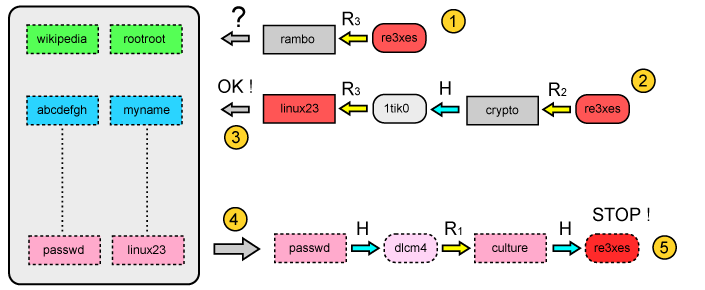
\includegraphics[width=15cm]{img/rain3}

\begin{itemize}
\item À partir d'une empreinte ("re3xes"), on calcule la dernière réduction utilisée dans la table et on
regarde si le mot de passe apparaît dans la dernière colonne de la table (étape 1)
\item Si le test échoue ("rambo" n'apparaît pas dans la table), on passe au point 2 où l'on calcule une
chaîne avec les deux dernières réductions.
\item Si ce test échoue à nouveau, on recommence avec 3 réductions, 4 réductions, etc. jusqu'à
trouver une occurrence du mot de passe dans la table. Si aucune chaîne ne correspond alors
l'attaque échoue.
\item Si le test réussit (étape 3, ici "linux23" apparaît en fin de chaîne et également dans la table), on
récupère le mot de passe à l'origine de la chaîne qui a abouti à "linux23". Il s'agit ici de
"passwd".
\item  On génère la chaîne (étape 4) et on compare à chaque itération l'empreinte avec l'empreinte
recherchée. Le test est concluant, on trouve ici l'empreinte "re3xes" dans la chaîne. Le mot de
passe courant ("culture") est celui qui a engendré la chaîne : l'attaque a réussi.
\end{itemize}
~\\
Afin d'éviter les collisions, on utilise plusieurs fonctions de réduction ($R_{1}, R_{2}, .., R_{n}$). On parle alors de rainbow tables. 

\subsubsection{Contre-attaque}

Afin d'éviter l'utilisation de tels tables, il suffit d'introduire un salt dans la fonction de hashage.

\subsubsection{Les faux positifs (false alarm)}
Étant donné un hash $C$ compris dans l'ensemble B, tell que $Y_1 = r(C)$, alors il est possible que la chaine
que nous reconstruisons lors de la recherche, converge sur la même valeur final $\frac{Ej}{Ys}$ d'une chaine de
notre table sans pour autant en faire partie: \\
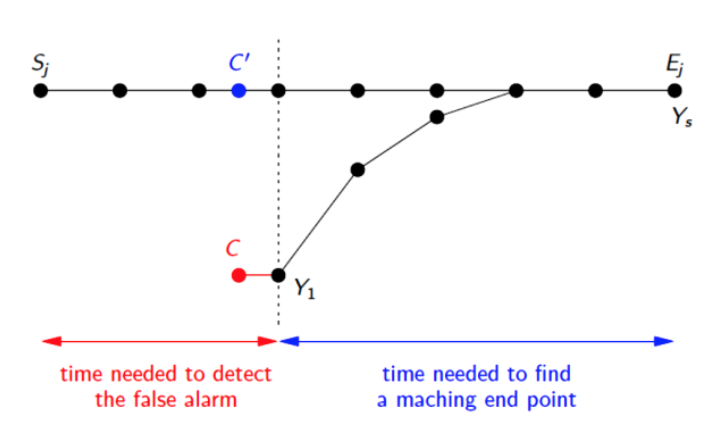
\includegraphics[width=10cm]{img/merge}
\\
Dans ce cas, l'algorithme détecte une valeur final commune à notre table (droite qui va de $S_j$ vers $E_j$) et
à la chaine (courbe qui va de $Y_1$ vers $Y_s$) que nous venons de reconstruire, il va alors falloir reconstruire
la chaine à partir du début ($S_j$) et au final se rendre compte que c'est un faux positif lorsqu'il arrive à
l'endroit où il devait trouver le hash recherché : $C' ≠ C$. \url{http://www.metu.edu.tr/~ccalik/timememory.pdf}

\subsection{Rainbow tables}
Les rainbow tables suivent le même principe que les tables de Hellman à la différence qu'elles n'ont
pas une seule fonction de réduction mais une variété en fonction de la longueur des chaines. Souvent
c'est un simple paramètre qui varie dans la fonction de réduction. Cela permet de les différencier selon
la position dans la chaine. Ainsi, dès à présent, si deux chaines rentrent en collision à des colonnes
différente, cela n'a pas d'effet sur la suite de la chaine, elles ne vont pas converger vers la même
valeur car leurs fonctions de réduction varient légèrement. Dans le cas où la collision se fait à la même
colonne, il est possible de le détecter car la valeur finale sera la même.
Une rainbow table parfaite est une table qui n'a aucune collision entre deux chaines à une colonne
donnée (qui ne se merge pas pour avoir au final, toutes les deux la même valeur de fin de chaine).


Quelque théorème:
\begin{itemize}
\item Avec $t$ et un nombre $N$ suffisamment grand, le nombre maximum de chaines normalement
requis pour une rainbow table parfaite (sans merge) est de : $m_{max}(t) ≈ \frac{2N}{t+1}$
\item Avec $t$ et pour un problème de taille $N$, le pourcentage de réussite espéré d'une rainbow table parfaite est de :
$P_{max}(t) ≈ 1- (1- \frac{2}{t+1}) )^{t}$
Qui tend vers $1-e^{-2}$ ≈ 86\% lorsque $t$ est grand.
\end{itemize}

\subsection{Conclusion}
TMTO n'est jamais meilleur qu'une attaque Brute force, mais il a du sens dans certain cas (attaque
répétée, temps limité pour l'attaque, etc).
Il faut bien analyser le problème avant de s'attaquer à celui-ci. 56-bit DES est par exemple impossible à
craquer : en brute force il faudrait 20 ans, avec TMTO 1 semaines, mais 8000 ans pour générer la table
(ainsi que 512Gb).
L'attaque consiste d'abord à pré calculer la table :
\begin{itemize}
  \item Éliminer les chaines qui se mergent.
  \item Paralléliser le calcul.
\end{itemize}
Puis vient l'attaque à proprement parler, la recherche du hash dans la table :
\begin{itemize}
  \item Paralléliser l'attaque.
  \item Pas besoin de beaucoup de mémoire.
\end{itemize}

% Il ne faut pas connaitre ce qu'il se trouve après
%\section{WEP}
%12.1 Introduction Wifi :
%Un point d'accès connecté via un câble au réseau. Plusieurs machines connectées via WIFI à ce point
%d'accès.
%Plusieurs manière : réseau ad hoc et mode infrastructure (cf cours de réseau). L'utilisation la plus
%simple et la plus courante des réseaux ad-hoc est faite par les réseaux sans fil Wi-Fi en permettant une
%mise en place rapide d'une connexion réseau entre deux ordinateurs.
%Les stations et le point d'accès communique via des ondes. (Non c'est vrai ?)
%Problème : n'importe qui peut capter/injecter des ondes avec une interface appropriée. (Record du
%monde : transmission de 382 km)
%War driving
%Un plouc peut se balader dans les rues en voitures et construire un carte des réseaux disponibles (un
%PC, un GPS et un bon software et le tour est joué).
%Security needs (en générale, valable pas uniquement pour le WEP)
%Vu que n'importe qui peut intervenir sur un réseau sans fil, on a besoin de s'assurer de trois choses :
%- L'authentification
%- L'intégrité des données
%- La confidentialité des données
%Authentification
%Plusieurs possibilités :
%- pas d'authentification : n'importe qui peut se connecter au réseau.
%c'est de moins en moins utilisé. Les providers donnent des boites contenant des clés par
%défaut. Il reste néanmoins certains endroits comme les cafés où on trouve des hots spots
%gratuits. A ne pas confondre avec les trucs de type FON.
%- Authentification via le SSID
%chaque modem broadcast son SSID. Tous les clients a porté peuvent découvrir le modem. On
%peut utiliser ce principe comme authentification : le client doit connaitre le SSID pour pouvoir
%se connecter. Pas du tout sécurisé car n'importe qui peut eavesdropper le SSID quand un client
%légitime se connecte.
%en pratique, il suffit de sniffer le réseau avec kismet ou Airodump.
%- MAC address authentification
%le routeur contient une liste de MAC adresses autorisées et vérifie si celle du client en fait
%partie. L'attaquant peut tjs sniffer une adresse MAC valable facilement. Il lui suffit de changer
%la sienne pour pouvoir se connecter au réseau. 3 lignes de commande en Unix :
%ifconfig INTERFACE down
%- 36 -
%-
%ifconfig INTERFACE hw ether NEW\_MAC\_ADR
%ifconfig INTERFACE up
%Authentification cryptée
%WEP ou WPA. C'est ce qui nous intéresse vraiment.
%WEP : wired equivalent privacy
%Le WEP fait partie du standard de l'IEEE 802.11 (standard de tout ce qui est réseau sans fil). Son but
%est de rendre les réseaux LAN aussi sécurisés que les réseaux câblés.
%Les grandes propriétés du WEP sont :
%- Pas de key management
%- Pas de protection contre les attaques replay
%- Authentification : une clé pour plusieurs utilisateurs
%- La confidentialité repose sur RC4 (stream cipher)
%- Dispose d'un system de vérification d'intégrité : CRC-32
%No key management
%Toutes les stations sans fils et le routeur ont la même clé pré-partagée. Cette clé est utilisée pour
%l'authentification et pour les encryptions.
%La clé est encodée manuellement sur chaque machine. Trop souvent, la clé entrée par le fabricant et
%n'est plus jamais modifiée.
%Replay attacks
%Vu que la clé n'est jamais changée, le méchant pirate peut attendre que le IV soit réutilisé et alors
%renvoyer un message qui est déjà passé. L'IV est sur 24 bits (16 777 216). Grace à notre ami le
%théorème des anniversaires, on sait qu'il y a 50% de chances qu'un IV se répète après 5000 paquets.
%Plusieurs solutions peuvent être implémentées pour éviter ca:
%- Nounce : challenge/réponse. A envoie un nonce (c.-à-d. un chiffre aléatoire fraichement
%généré). B l'encrypte et l'envoie à A. A vérifie que c'est bon.
%- Timestamp : A envoie son message accompagné d'un MAC (message authentification code : ça
%sert à être sûr de l'intégrité du message. Prenez le cours de crypto si vous voulez en savoir
%plus)
%- Sequence number : A et B discute en incrémentant un compteur.
%-
%Intégrité
%L'intégrité est assurée via CRC (contrôle de redondance cyclique). Cependant, CRC est designé pour
%détecter les erreurs de transmissions (erreurs aléatoires) mais pas les erreurs intelligentes des pirates.
%- 37 -
%Schéma d'encryptions
%La figure ci-dessous présente le schéma d'encryptions.
%On entre un message m. Celui-ci est coupé en byte mi et encodé via un xor avec le keystream.
%Le keystream est généré par RC4.
%RC4 est un stream cipher orienté byte. Il est donc très efficient en software (10x plus rapide que DES)
%et a l'avantage d'être simple. Il se passe en deux phases : l'initialisation et la génération de clé.
%Initialisation \& scrambling
%RC4 comporte un registre principal: le registre d'état (N=256 bytes). Il est noté S dans la suite
%La clé et le vecteur d'initialisation servent à initialiser un second registre le registre K.
%Dans un premier temps, le tableau S est rempli des 0->N-1.
%Ensuite, le tableau est mélangé avec le registre de K de la manière suivante.
%Génération de clé
%Vient ensuite la génération de clé: elle est faite de la manière suivante :
%Maintenant que nous connaissons le fonctionnement du WEP, nous pouvons passer à
%l'authentification cryptée.
%- 38 -
%Je crois que l'image en dit suffisamment long. C'est comme d'habitude un challenge/réponse.
%12.2 Attaque contre le WEP :
%1ere attaque : Exhaustive search
%WEP: 40bits de clé + 24 bits de IV = 64 bits  264 bits c'est encore faisable avec un gros gros pc.
%Il existe des versions de WEP avec 104 bits de clé +24 bit d'IV. Là c'est plus possible.
%2eme attaque : CRC property
%CRC a une sale propriété : CRC est linéaire par rapport au XOR c.-à-d. que
%Ça craint vachement !
%Je m'explique : un attaquant connait l'adresse ip contenue dans le message M. Il peut calculer un ∆m
%tel que m xor ∆m = l'adresse ip du pirate. Il lui suffit ensuite de calculer CRC(∆m) et de xor le tout.
%L'attaquant a réussi à modifier un message sans connaitre la clé K tout en gardant l'intégrité du
%message.
%3eme attaque : Keystream Reused
%Comme dit précedement, le IV fait 24 bits=3bytes.
%Vu que les gens changent jamais de clé, un keystream donnée (cad un IV) revient relativement
%souvent.
%En général l'IV est un compteur. Il est donc possible de forcer la réutilisation d'un IV en reboutant le
%routeur (compteur réinitialisé). Il y a 50% de chances de revoir passer un IV dans 212 paquets (birthday
%paradox).
%Si on connait un message qui a été encrypté avec un certain IV, on peut retrouver un autre message
%encrypté avec un même IV.
%C= K xor M
%C'=K xor M'  M' = C' xor C xor M
%A nouveau pas besoin de la clé.
%on peut facilement connaitre un message M( entête de paquets connus, etc)
%4eme attaque : Cryptanalyse
%C'est ici que les choses marantes commencent !
%2 ans après la sortie de WEP, on commence à piger que y des IV qui font tout foirer. Ils permettent de
%retrouver certains états internes du registre S dont je vous parlais précédemment et parfois même la
%clé complète.
%Pour réaliser cette attaque, on doit connaitre l'IV et les premiers bytes d'un message et de son chiffré.
%(L'IV est envoyé en clair et le chiffré est sniffé)
%Le message est encrypté avec la clé (IV||key) = (K0, K1, K2, K3, K4,..., K7) = (3,255, X, K3,..., K7)
%- 39 -
%Donc l'IV est (3, 255, X) et X est supposé connu.
%On effectue les quatre premières étapes de l'initialisation :
%On suppose pour un instant que on s'arrete ici pour l'initialisation.
%Si on doit encoder un truc à ce stade, le keystream généré sera 6+X+K3 :
%Comme le keystream est connu, on peut trouver K3 pour i=3
%Cependant, on ne peut pas arrêter l'initialisation au 4eme stade.
%Quelle est la probabilité que les éléments 0,1 et 3 du tableau ne soient pas modifiés dans le reste de
%l'initialisation? Apparemment c'est
% .
%Donc si on voit suffisamment de IV, on finira bien par en trouver un qui fera l'affaire.
%Une fois que K3 est connu, on refait la même chose avec un autre IV :
%Si IV = {4, 255, X}, on peut effectuer la même démarche. On trouve alors pour i=4,
%On peut donc trouver toute la clé byte par byte en continuant.
%En moyenne, il faut 4millions de IV pour retrouver une clé de 128 bits. Le nombre de IV nécessaire est
%linéaire en fonction de la longueur de clé (-> très mauvais).
%Further attacks
%Il existe des attaques du même styles mais plus puissantes mais elles ne sont (heureusement) pas
%détaillées dans le cours.
%
%\section{WPA}
%\subsection{WPA}
%Le WPA ou « Wifi protected access » a pour but de remplacer le WEP. Comme vous avez pu le voir, le
%WEP c'est de la merde. Ce remplacement est un patch assez urgent avant la publication de WPA2
%(802.11i).
%Depuis 2003, tous les appareils Wifi doivent implémenter le WPA.
%Propriétés-
%-
%-
%-
%-
%-
%et amélioration par rapport au WEP
%Un compteur est utilisé pour éviter les attaques par répétition.
%L'IV est sur 48 bits
%Chaque utilisateur est authentifié contrairement au WEP ou les machines seulement sont
%identifiées.
%Les clés sont dynamiquement rafraichies en utilisant TKIP.
%AES est utilisé dans WPAE au lieu de RC4 dans WEP et WPA2
%Il existe deux modes de fonctionnement du WPA :
%o Personnal : on utilise alors des « pre-shared key » (PSK)
%chaque appareil connecté utilise le même mot de passe de 256 bits.
%Cette clé peut être saisie soit sous forme de chaîne de 64 chiffres hexadécimaux, ou
%comme une phrase de passe de 8 à 63 caractères ASCII imprimables. Si les caractères
%ASCII sont utilisés, la clé de 256 bits est calculée en appliquant la fonction de
%dérivation de clé PBKDF2 au mot de passe, en utilisant le SSID comme le sel de 4096
%itérations de HMAC-SHA1. L'authentification de se fait via EAP-MD5. (MD5 +
%Extensible Authentication Protocol voir plus loin)
%o Entreprise : on utilise l « IEEE802.1x Authentification Server »
%chaque utilisateur doit s'identifier. On a besoin d'un serveur qui gère tous les comptes
%des utilisateurs (genre Radius)
%http://en.wikipedia.org/wiki/IEEE\_802.1X
%13.2 Architecture et protocoles :
%On considère 3 acteurs :
%- Le client (supplicant)
%- Le point d'accès (authentificateur)
%- Le serveur d'authentification
%- 41 -
%Il y a quatre phases importantes
%- L'accord sur la politique de sécurité
%- L'authentification
%- La génération de clé et leur distribution
%- La confidentialité et l'intégrité des données
%Phase 1 : L'accord sur la politique de sécurité
%Phase 2: l'authentification
%Pour l'authentification, comme dit précédemment EAP est utilisé.
%EAP n'est vraiment un protocole d'authentification en lui-même. Seul, il ne sert à rien. Il a été créé
%pour transporter les messages selon un cadre bien défini. Il contient 4 sortes de message : request,
%response, succes et failure. Les paquets request sont émis par l'authentificateur (Acces Point). Le
%suppliant doit y répondre correctement afin de recevoir un paquet succes.
%- 42 -
%L'AP peut envoyer autant de paquets request qu'il a envie avant d'accorder ou non l'accès.
%EAP est utilisé avec plusieurs outils :
%- Legacy based methods : EAP-MD5
%- Méthodes basées sur un certificat : EAP-TLS, EAP-TTLS, PEAP
%- Méthodes basées sur des mots de passe : LEAP, SPEKE
%- ...
%EAP-MD5
%Utilisé uniquement en mode Personnal WPA.
%L'authentification se fait via le hash d'un challenge et du mot de passe. Cependant, MD5 est
%absolument plus suffisant de nos jours. Cette méthode n'est PAS sécurisée.
%Comme le dit Wikipédia: It offers minimal security; the MD5 hash function is vulnerable to dictionary
%attacks, and does not support key generation, which makes it unsuitable for use with dynamic WEP, or
%WPA/WPA2 enterprise.
%EAP-TLS
%EAP est utilisé avec le TLS. EAP se base sur les PKI (public key infrastructure -> certificat) pour sécuriser
%les communications entre le serveur d'authentification (AS). L'authentification est donc très fortement
%sécurisée mais nécessite la mise en place des PKI.
%Le client et le serveur ont un certificat.
%L'EAP-TLS est donc essentiellement utilisé en entreprise.
%EAP-TTLS
%C'est grosso modo la même chose sauf qu'ici il n'y a que l'AS qui a un certificat. On peut utiliser une
%méthode d'authentification moins sécurise pour le client (CHAP ou PAP)
%-
%-
%PAP : Password authentication protocol
%Quand l'AS te demande d'envoyer ton pass, tu l'envoies.
%CHAP: Challenge-Handshake Authentication Protocol
%lorsque tu reçois un challenge, le prouveur encrypte le challenge avec sa clé et envoie le chiffré
%au vérifieur
%- 43 -
%Phase 3 : key dérivation
%4 way hands shake:
%http://en.wikipedia.org/wiki/IEEE\_802.11i-2004 -> c'est bien expliqué dans le cours y a que dale.
%The Master Key key is designed to last the entire session and should be exposed as little as possible.
%Therefore the four-way handshake is used to establish another key called the PTK (Pairwise Transient
%Key). The PTK is generated by concatenating the following attributes: PMK, AP nonce (ANonce), STA
%nonce (SNonce), AP MAC address, and STA MAC address. The product is then put through PBKDF2-
%SHA1 as the cryptographic hash function.
%The handshake also yields the GTK (Group Temporal Key), used to decrypt multicast and broadcast
%traffic.
%1.2.3.4.The AP sends a nonce-value to the STA (ANonce). The client now has all the attributes to
%construct the PTK.
%The STA sends its own nonce-value (SNonce) to the AP together with a MIC, including
%authentication, which is really a Message Authentication and Integrity Code: (MAIC).
%The AP sends the GTK and a sequence number together with another MIC. This sequence
%number will be used in the next multicast or broadcast frame, so that the receiving STA can
%perform basic replay detection.
%The STA sends a confirmation to the AP.
%- 44 -
%As soon as the PTK is obtained it is divided into five separate keys:
%PTK (Pairwise Transient Key – 64 bytes)
%1. 16 bytes of EAPOL-Key Confirmation Key (KCK)– Used to compute MIC on WPA EAPOL Key
%message
%2. 16 bytes of EAPOL-Key Encryption Key (KEK) - AP uses this key to encrypt additional data sent
%(in the 'Key Data' field) to the client (for example, the RSN IE or the GTK)
%3. 16 bytes of Temporal Key (TK) – Used to encrypt/decrypt Unicast data packets
%4. 8 bytes of Michael MIC Authenticator Tx Key – Used to compute MIC on unicast data packets
%transmitted by the AP
%5. 8 bytes of Michael MIC Authenticator Rx Key – Used to compute MIC on unicast data packets
%transmitted by the station
%Pour ceux qui veulent comparer avec le schéma du cours :
%- 45 -
%1.2.GEK (Group Encryption Key): Key for data encryption (used by CCMP for authentication and
%encryption and by TKIP).
%GIK (Group Integrity Key): Key for data authentication (used only by Michael with TKIP)
%Group key Hands shake
%The GTK used in the network may need to be updated due to the expiry of a preset timer. When a
%device leaves the network, the GTK also needs to be updated. This is to prevent the device from
%receiving any more multicast or broadcast messages from the AP.
%To handle the updating, 802.11i defines a Group Key Handshake that consists of a two-way handshake:
%1. The AP sends the new GTK to each STA in the network. The GTK is encrypted using the KEK
%assigned to that STA, and protects the data from tampering, by use of a MIC.
%2. The STA acknowledges the new GTK and replies to the AP.
%En gros à partir de la clé principale (master key), la station et l'AS vont générer toute une série de clé.
%Chaque clé est utilisée dans un but différent. Le schéma ci-dessous explique bien les relations entre ces
%différents clés.
%- 46 -
%Phase 4 : data integrity
%Deux algorithmes possibles peuvent être utilisés avec WPA :
%- TKIP : RCA+ MIC
%- CCMP : AES en mode compteur (WPA2 uniquement)
%TKIP: key mixing scheme and encryption
%MIC
%Mic utilise l'algorithme de Michael a la place de CRC32. Michael est utilisé avec une clé. Pourquoi
%Michael ? Simplement parce que c'était le plus puissant des MIC compatible avec les vieilles cartes.
%A cause des faiblesses de Michael, le réseau est coupé pendant une minute si 2 frames ne passent pas
%le check de Michael. Ensuite, des nouvelles clés doivent être régénérées.
%- 47 -
%13.3 Attaques :
%Attaque sur PSK
%Toutes les clés dérivent de la PSK :
%PMK = PBKDF2(SSID,PSK) suivi d'un 4-way hands shake.
%Sachant qu'on peut écouter ce hand shake, on peut tester toutes les clés possibles :
%Procédure :
%Pour chaque candidat de mot de passe, on calcule le PMK associé.
%On calcule ensuite la PTK
%Et finalement le MIC et on le compare avec celui qu'on a écouté.
%Il existe des rainbows tables pré calculée pour les 1000 SSID les plus courants.
%Attaque sur TKIP
%-
% injection de paquets
%-
% Décryptions de paquets de l'AP vers le client
% \subsection{Conclusion}
%Glossaire:
%
%\section{IPsec}
%Protéger les données au network layer avec Virtual Private Networks (VPNs) construits avec IPSec
%(Internet Protocol Security).
%14.1 VPN :
%Les VPNs permettent d'étendre un réseau privé à travers un réseau public.
%Applications: Interconnexion de sites distants à travers Internet, accès au réseau de l'entreprise à
%partir d'un ordinateur connecté à Internet comme si on était à l'entreprise.
%Mécanisme :
%\begin{itemize}
%  \item 2 sets d'adresses : IP public pour échanger des données sur Internet et des adresses privées
%qui routent les paquets entre les hôtes sur le réseau privé.
%  \item Encapsulation : le paquet est encapsulé dans un paquet IP pour son voyage sur Internet.
%  \item Encryption : pour éviter le eavesdropping et les modifications de données sur le réseau
%public.
%\end{itemize}
%Protocoles :
%\begin{itemize}
%  \item PPTP (Point to Point Tunneling Protocol) : développé par Microsoft.
%  \item L2TP (Layer 2 Tunneling Protocol) : développé par IETF, rassemble L2F de Cisco et PPTP de
%Microsoft.
%  \item IPSec (IP Security) : développé par IETF.
%\end{itemize}
%14.2 IPSec :
%Le standard est ouvert et extensible. Des algorithmes publics sont utilisés pour la confidentialité,
%l'authentification et l'intégrité.
%14.2.1 Modes d'opération :
%\begin{itemize}
%  \item Transport : les données sont encryptées et/ou authentifiées. La sécurité est faite de
%manière end-to-end.
%  \item Tunnel : tout le paquet est encapsulé dans un nouveau paquet. La sécurité peut être faite
%par les routeurs intermédiaires.
%Chaque routeur contient une Security Policy Database qui défini quel paquet doit être sécurisé
%en fonction de sa destination et de sa source par exemple (e.g. : sécuriser le trafic telnet,
%UDP,...)
%\end{itemize}
%14.2.2 Protocole d'échange de clés :
%Internet Key Exchange (IKE) :
%Protocole permettant l'installation d'un tunnel sécurisé entre partenaires.
%Objectifs :
%\begin{itemize}
%  \item Authentification du partenaire
%  \item Echange de clé entre partenaires
%  \item Négociation du paramètre
%\end{itemize}
%- 51 -
%Phases :
%1. Négocier un IKE SA (Internet Key Exchange Security Association) pour protéger les négociations
%\begin{itemize}
%  \item Authentification : pre-shared secret (PSS), clés asymétriques, utiliser la clé publique
%d'une certification authority (X.509)
%  \item Echange de clés : clés générées avec Diffie-Hellman
%  \item Négocier le paramètre
%\end{itemize}
%o Main mode : clé de session générée avec Diffie-Hellman (plein de paramètres) and
%utilisée pour protéger le reste de la transaction (négociation du paramètre et
%authentification).
%
% un eavesdropper ne sait pas dire l'identité des paires.
%o Agressive mode : piggyback sur l'étape d'authentification pour l'échange de Diffie-
%Hellman, les identités et le pwd hash sont envoyés en clair. MAIS ne doit échanger
%que 3 paquets !
%
% attaquable (CKY cookie dans les headers des paquets IKE)
%2.Définir les besoins du SA (Security Association) pour les flux ESP (Encapsulated Security
%Payload) ou AH (Authetification Header)
%Quick mode :
%\begin{itemize}
%  \item Sans Perfect Forward Secrecy (PFS) :
%o Les session keys sont rafraichies périodiquement (1h)
%o Les session keys sont issues du même secret
%o Voler ce secret compromet toutes les clés
%  \item Avec PFS
%o A chaque nouvelle session key, on fait un Diffie-Hellman (plus lent)
%o Voler 1 clé ne compromet pas les clés précédentes
%\end{itemize}
%Security Association :
%Avant de pouvoir échanger des paquets en toute sécurité, les ordinateurs doivent établir une
%Security Association (SA) en utilisant IKE.
%Pour chaque communication sécurisée, le SA mémorise les algorithmes, les clés, la période de
%validité des clés, le numéro de séquence et l'identité du partenaire.
%Il faut 1 SA pour chaque flux unidirectionnel : une connexion TCP demande un SA pour chaque
%direction. (1 SA par destination par protocole, par port).
%Les SAs sont identifiés par un Security Parameter Index (SPI) :
%\begin{itemize}
%  \item La source indique le SPI sur tous les paquets qui sont envoyés (elle décide quels paquets
%doivent être exécuté avec quel SA)
%  \item La destination utilise le SPI pour trouver le SA qui décrit comment traiter ce paquet.
%\end{itemize}
%14.2.3 Protocole sécurisé :
%Authentication Header (AH)
%Pour vérifier l'authenticité et l'intégrité du paquet.
%- 52 -
%L'authentification est calculée sur base de :
%\begin{itemize}
%  \item Données qui suivent le AH
%  \item Le header (mis à 0 quand il faut calculer l'information d'authentification)
%  \item Les champs importants dans l'IP header : source, destination, protocol, length, version,...
%  \item Les champs exclus de l'IP header : type of service, flags, fragment offset, TTL, header
%checksum.
%\end{itemize}
%L'algorithme utilisé pour générer les données d'authentification est négocié à la création du SA.
%
% utilise le HMAC : sécurité démontrable, peut être utilisé avec n'importe quelle hash function,
%maintient les performances de la hash function originale :
%HMAC(K,m) = H( (K xor opad) || H((K xor ipad) || m) )
%HMAC-SHA1-96 signifie HMAC calculé avec H=SHA1 et la sortie tronquée à 96 bits.
%Encapsulated Security Payload (ESP)
%Pour l'encryption et l'authentification du paquet.
%L'encryption est seulement faite sur l'encapsulated data et le trailer (à la fin du paquet). PAS
%d'encryption sur les champs du header, ni sur les données d'authentification.
%L'authentification (optionnelle) est faite sur l'ESP header et tout ce qui suit MAIS PAS sur l'IP
%header (différence avec AH).
%Exemple d'algorithme :
%\begin{itemize}
%  \item Encryption : DES-CBC, NULL
%  \item Authentification : HMAC-SHA-96, HMAC-MD5-96, NULL
%\end{itemize}
%NULL ne peut pas être utilisé dans le même SA pour l'encryption et l'authentification.
%14.2.4 IPSec avec NAT
%AH : que ça soit en mode transport ou tunnel, AH authentifie l'IP header et donc ne
%permet pas au NAT de modifier l'IP source sans provoquer une perte d'intégrité.
%ESP :
%\begin{itemize}
%  \item Mode transport : en TCP ou UDP, les headers sont encryptés et donc le checksum ne peut
%pas être mis à jour
%  \item Mode tunnel : le checksum TCP ou UDP fait référence à l'IP header interne, qui n'est pas
%modifié par le NAT.
%\end{itemize}
%
% ESP en mode tunnel est le seul moyen de traverser un NAT !
%- 53 -
%Sécurité au transport layer.
%15. SSL :
%15.1 SSL
%SSL = Secure Socket Layer à été développé par NetScape
%15.1.1 Applications
%\begin{itemize}
%  \item Créer un nouveau protocole à partir d'un protocole existant : HTTP -> HTTPS
%o Désavantage : seuls les clients supportant TLS peuvent se connecter
%o Avantage : sur que la communication est sécurisée
%  \item Etendre un protocole pour négocier SSL/TLS : demander TLS avec STARTTLS
%o Avantage : le client ne doit pas forcément supporter TLS pour utiliser le service
%\end{itemize}
%Exemples :
%\begin{itemize}
%  \item HTTPS :
%o L'utilisation de TLS n'est pas négociable
%o Garanti la confidentialité et l'authenticité des données transmises
%o Le server doit avoir un certificat
%o Le client peut en avoir un (e.g. : eBanking)
%  \item Mail
%o ESMTP, POP3, IMAP transmettent par défaut le mot de passe en clair
%o TLS protège le mot de passe et le contenu du mail
%\end{itemize}
%15.2 TLS
%TLS = Transport Layer Security (version actuelle de SSL). Se situe entre l'application et le network layer.
%- 54 -
%15.2.1 Record Layer
%Traitement des données
%\begin{itemize}
%  \item Fragmentation
%  \item Compression (optionnel)
%  \item Authentification (MAC)
%  \item Encryption
%\end{itemize}
%Transmets les fragments traités au transport layer
%Une fois, transmis, les opérations inverses sont effectuées.
%MAC :
%MAC= hash ( MAC\_key || Pad2 ||
%
%hash(MAC\_key || Pad1 || Seq\_Nb || Length || Content))
%- MAC\_key: secret shared by client and server.
%- Pad1: constant character 0x36 repeated 48 times (if MD5) or 40 times (if SHA1).
%- Pad2: constant character 0x5c repeated the same number of times.
%- Seq\_Nb: sequence number of this message.
%- Hash: Either HMAC-MD5 or HMAC-SHA1
%- Length: Length in bytes of the compressed record.
%- Content: Compressed record.
%Encryption :
%Faite sur des records compresses et authentifiés.
%Soit avec du chiffrement par blocs:
%o DES (40 bits ou 56 bits), 3DES, IDEA, RC2 (40 bits)
%o AES (128 bits ou 256 bits) dans TLS v1.1 (256 bits pour les mails UCL)
%Soit avec du chiffrement en flux:
%o NULL, RC4 (40 bits ou 128 bits)
%
% le client doit refuser des clés de 40 bits si cette longueur est suggérée par le serveur.
%15.2.2 Handshake protocol
%Négociation de:
%- protocole version (SSL 3.0, TLS 1.0, TLS 1.1).
%- algorithmes:
%o Key exchange (RSA, Diffie-Hellman).
%o Encryption (DES, 3DES, IDEA, RC4, RC2, AES).
%o MAC (HMAC-MD5, HMAC-SHA).
%- Le client propose les algorithmes par ordre de préférence, le serveur choisi.
%- Authentification optionnelle du partenaire en utilisant un certificat.
%- Les messages ne sont pas cryptés.
%- Le dernier message authentifie l'échange.
%- 55 -
%
%Client\_Hello : utilisé par le client pour initialiser une connexion SSL (envoyé en clair sans
%signature)
%o Crypto : liste des algorithmes cryptographiques supportés (Authentication + key
%exchange + cipher + hash).
%Content:
%-
%-
%-
%-
%-
%-
%Protocol Version.
%32 bytes long random number.
%Composed of two parts:
%o 4 bytes Unix time (number of seconds since 01/01/1970)
%o 28 bytes random number
%Optional Session Identifier.
%o Each SSL session has an identifier which can be used later to restart a
%session.
%List of supported Ciphers.
%
%List of supported Compression Methods.
%\begin{itemize}
%  \item Server\_Hello : réponse du serveur (envoyé en clair sans signature)
%\end{itemize}
%Content:
%-
%-
%-
%-
%-
%Protocol version: highest version of the protocol supported by both client and
%server.
%Random number.
%Optional Session Identifier, if it allows sessions to be resumed.
%Cipher Suite: One of the cipher suites proposed by client.
%Compression Method.
%- 56 -
%
%Server\_Certificate : le serveur s'authentifie (un serveur peut avoir plusieurs certificats à partir
%de différentes certification authorities). Le certificat peut aussi être envoyé par le client quand
%l'identification du client est demandée par le serveur avec Certificate\_Request.
%Content:
%-
%A list of X.509 certificates:
%o Server certificate.
%o Certificates of certification authorities if any.
%
%
%Server Hello\_Done : indique que le serveur a fini la 1ere phase du handshake (envoyé non
%crypté).
%Client\_Key\_Exchange : utilisé par le client pour envoyé le PreMasterSecret (encrypté avec la
%clé publique du serveur).
%o Utilise des nonce de 32B et un masterSecret de 48B
%Content:
%-
%Encrypted PreMasterSecret with the public key of the server.
%
%
%Change\_Cipher\_Spec :
%o Utilisé par le client et le serveur pour signaler qu'il vont utiliser une nouvelle clé.
%o Durant le handshake, indique que le prochain message sera encrypté avec la clé
%appropriée.
%Handshake\_Finished :
%o Envoyé par le client et le serveur pour confirmer l'établissement d'une session SSL
%sécurisée. (Sécurisée ssi le client et le serveur ont reçu ce message).
%o Permet de détecter les man in the middle attack sur des messages Client\_Hello et
%Server\_Hello (e.g.: proposer un chiffrement plus faible).
%o Premier message encrypté dans chaque direction.
%Content:
%-
%-
%Keyed hash (MD5 or SHA-1) of all the handshake messages and the
%MasterSecret.
%
%\section{Kerberos}
%1.1 Motivation :
%Parfois plusieurs utilisateurs veulent avoir l'accès à plusieurs serveurs sur un même réseau. Une
%solution pour gérer la sécurité de l'authentification est que chaque serveur retienne les mots de passe
%de chaque utilisateur. Cette approche n'est cependant pas idéale :
%\begin{itemize}
%  \item Elle n'est pas sure. Un seul serveur compromis peut compromettre tous les utilisateurs.
%  \item Elle est inefficace. Les mots de passes doivent chaque fois être changés sur tous les serveurs.
%  \item Elle n'est pas pratique. Les mots de passes doivent être entrés pour chaque requête.
%\end{itemize}
%Dès lors, il est plus raisonnable de centraliser les informations. Kerberos permet cela.
%1.2 Kerberos :
%Kerberos est un protocole d'authentification réseau qui repose sur un mécanisme de clés secrètes
%l'utilisation de tickets. Il est basé sur de la cryptographie à clef symétrique. Une fois que
%l'authentification est faire, on peut accéder au réseau sans devoir redonner son mot de passe ou nom
%d'utilisateur.
%1.3 Elements principaux :
%Kerberos utilise tous les éléments suivants :
%\begin{itemize}
%  \item Un client C. C'est la personne qui veut se connecter au réseau.
%  \item Un serveur d'authentification AS 1. Ce serveur va fournir au client un premier ticket (TGT 2 ), au
%client qui en fait la demande.
%  \item Un serveur de ticket (TGS 3). Une fois qu'un client présente son ticket à ce serveur, ce dernier
%peut lui donner un autre ticket pour accéder à certaines ressources.
%  \item un serveur S dont le client veut avoir l'accès. Pour avoir l'accès à ce serveur, le client doit avoir
%le ticket correspondant fourni par le TGS.
%Au final, pour qu'un client ait accès au serveur S, il doit avoir son ticket ainsi qu'un authentifiant.
%Le ticket contient les informations suivantes
%  \item Ic, l'identité du client.
%  \item v, la période de validité du ticket.
%  \item Kc,s, la clef symétrique de session à utiliser entre le client et le serveur.
%  \item D'autres trucs comme des flags, l'adresse IP, etc.
%\end{itemize}
%Ce ticket est encryptée avec la clef Ks du serveur. L'authentifiant est juste l'identité du client (Ic) suivi
%d'un timestamp t. Regardons à présent tous les messages échangés pour obtenir ce fameux ticket. Le
%schéma ci dessous reprend l'ensemble des échanges.
%Analysons les séparément.
%1. Authentication server.
%2. Ticket-granting ticket.
%3. Ticket granting server.
%- 58 -
%1.3.1 Echange entre le client et AS:
%Le client doit être authentifié pour pouvoir accéder au TGS. Dès lors, il va en tout premier lieu faire une
%demande d'authentification à AS. Ce dernier va lui renvoyer un TGT encrypté avec la clef du TGS ainsi
%qu'une clef de session encryptée avec la clef de C. Plus particulièrement, on a les messages suivants :
%1. Ic, ITGS,N. Le client envoie à AS son identité, celle du TGS dont il veut faire une requête, ainsi
%qu'un nonce utilisé pour éviter les replay attaques.
%2. {ITGS,N,KC,TGS}KC , {IC, v,KC,TGS}KTGS . Le premier bloc peut être décrypté par le client pour
%qu'il puisse le KC,TGS nécessaire pour la suite du protocole. Le deuxième bloc ne peut être
%décrypté que par le TGS.
%1.3.2 Echange entre le client et TGS:
%Une fois le TGT reçu, le client va envoyer une requête au TGS. Le TGS va alors utiliser la clef de session
%pour vérifier le ticket. Il peut alors voir si le client est autorisé à accéder au serveur S.
%Si oui, il va donner au client un ticket lui accordant ce service. Pratiquement, on a les messages
%suivants
%1. Is,N0, {IC, v,KC,TGS}KTGS , {IC, t}Kc,TGS . On a l'identité du service voulu, un nounce, le TGT
%ainsi que d'autres données encryptées avec la clef KC,TGS entre le client et le TGS et qui
%comprend l'identité du client et un timestamp.
%2. {IS,N0,KC,S}KC,TGS , {IC, v,KC,S}Ks . Le TGS répond un message pouvant être décrypté par le
%client et qui contient une clef de session avec le service S, et un autre message ne pouvant être
%décrypté que par S.
%1.3.3 Echange entre le client et S:
%Finalement, le client va demander l'accès au serveur S à travers les messages suivants
%1. {Ic, v,KC,S}KS , {IC, t}KC,S . Le client envoie son ticket de service ainsi qu'un autre message que
%le serveur ne pourra décrypter que quand il aura obtenu le KC,S. Il pourra alors voir que les
%deux Ic correspondent bien.
%2. {t}KC,S . Le serveur lui renvoie simplement un timestamp que le client peut décrypter.
%Le client peut maintenant accéder au serveur !
%1.4 Commentaires :
%Avec Kerberos, la responsabilité de stocker les tickets revient exclusivement au client. Par
%ailleurs, une fois qu'un client a eu son authentification (il la garde environ 8 heures), il ne doit plus
%contacter AS. Il peut accéder aux autres services même si ce dernier est down. Et il est finalement
%impossible de révoquer le ticket d'un client qui a été authentifié.
%
%\section{PGP}
%Pretty Good Privacy (PGP) est un logiciel de chiffrement et de déchiffrement cryptographique.
%Il garantit la confidentialité et l'authentification pour la communication des données. Il est le plus
%souvent utilisé pour la signature de données, et sa gestion des clefs.
%17.1 Encryption hybride :
%PGP utilise pour encrypter les données à la fois des clefs asymétriques et symétriques, comme
%le montre le schéma suivant.
%Le système est donc hybride. Pour chiffrer un document, PGP utilise une clef symétrique aléatoire (clef
%de session). Ensuite, PGP chiffre la clef de session avec la clef publique du destinataire.
%Cela à d'une part l'avantage d'être rapide, au lieu de crypter l'entièreté du document avec la clef
%publique (fort lent), on ne l'utilise que pour crypter la clef de session qui est nettement plus petite, et
%d'autre part, le problème de distribution des clefs est réglé puisque la symétrique est encryptée. Pour
%l'encryption symétrique beaucoup d'algorithmes peuvent être utilisés (TDES, IDEA, AED, etc.), pour
%l'asymétrique on utilise généralement le RSA ou l'Elgamal qui se base sur le problème du logarithme
%discret.
%17.2 Signature de la clef publique :
%Pour la signature, on utilise généralement l'algorithme DSA ou RSA. L'Elgamal n'est plus
%recommandé du fait qu'une attaque a révélé que les clefs Elgemal n'étaient plus sûre lors qu'elles sont
%utilisées pour l'encryption et pour la signature. De manière générale, il ne faut jamais utiliser la même
%clef pour plusieurs choses.
%17.3 Protection des clefs privées :
%Les clefs privées sont encryptées sur le disque de l'utilisateur avec un algorithme se basant sur
%une passphrase. Quand la clef est nécessaire, l'utilisateur utilise sa passphrase pour déchiffrer sa clef.
%Cependant, pour préserver la sécurité, et respecter le principe du maillon le plus faible, la passphrase
%doit être choisie intelligemment de sorte qu'elle soit aussi solide que les clefs utilisées pour la
%signature ou l'encryption. Le tableau ci dessous reprend une correspondance de taille entre les clefs
%symétriques et asymétriques pour avoir une même solidité.
%- 60 -
%17.4 Validité des clefs publiques :
%Comment être sur qu'une clef qu'on utilise pour chiffrer un message est la clef correcte ? Une
%manière sûre de vérifier cela, est de faire une rencontre IRL, vérifier l'identité de la personne, vérifier
%le hash de la clef, et puis seulement signer la clef. En procédant comme cela, on peut être sûr que
%la clef n'a pas été modifiée par la suite. On peut aussi utiliser des certificats.
%17.5 Distribution des clefs publiques :
%Il y a deux notions importances dans PGP.
%1. La validité : Je sais à qui appartient cette clef.
%2. La confiance : Je sais que cette personne ne signe pas des clefs n'importe comment.
%Quand on signe une clef, on déclare sa validité. Sachant cela, on peut former un graphe dirigé
%où les sommets correspondent aux différentes personnes et où les arêtes A ! B signifient que A a validé
%la clef de B. On met aussi des poids sur les arêtes, 1 si A fait entièrement confiance à B, et 0.5 s'il lui
%fait partiellement confiance. Dès lors, une personne peut considérer les clefs d'autres personnes
%comme valide si d'une part, elle fait totalement confiance à une personne qui a vérifié l'adresses de
%ces autres personnes (A fait confiance à B, et B a validé la clef de C : La clef de C est valide pour A) , ou
%si d'autre part, elle fait moyennement confiance à plusieurs personnes qui ont vérifié la clef (A fait
%moyennement confiance à B et C, mais B et C ont tout deux validé la clef de D : le clef de D est valide
%pour A).
%17.6 Révocation de clef :
%Une manière naïve de procéder est de simplement enlever la clef du serveur. Cependant, il se
%peut que la clef a été dupliquée sur d'autres serveurs, que des personnes l'aient téléchargée, etc.
%On doit donc procéder autrement. On peut créer un certification de révocation de la clef quand on
%génère cette dernière. On l'envoie alors sur le serveur PGP quand on veut révoquer la clef. Pour bien
%faire, il faut aussi l'envoyer aux correspondants réguliers. Par ailleurs, lors de la génération d'une clef,
%on met une limite de validité qui fait que la clef expire après cette date.
%
%
\end{document}
